\chapter{Datentypen und Methodenklassen}

%\section{Einleitung}

räumlich (gebietlichen, regionalen, lokalen, örtlich, mehrdimensionalen, Raumordnung, Lagebeziehung, Raum-, Orts-, Lage-, Flächen-) \\

räumlich verteilte Positionen (Standorte, Lokationen, Stellen, Lageparameter) \\
diskrete Raumzonen \\

an Positionen beobachtete Daten (Ausprägungen, Zielwerte, Attributsrealisierung) 

\section{Besonderheiten räumlicher Daten}

\subsection*{Räumliche Assoziation?}
\label{subsec:tobler}

Abbildung \ref{fig_densitymaps} verdeutlicht das Konzept räumlicher Autokorrelation. Die starke Präsenz von räumlicher 
Abhängigkeit verkompliziert die Analyse, da nicht von unabhängigen Daten ausgegangen werden kann. Abb 3.2 zeigt grob auf,
welches Erscheinungsbild eine (über Verwaltungskreise) zufällig verteilte Bevölkerung aufwiese.

\begin{figure}[htb] %h=here, t=top, b=bottom, p=page of float
    \centering %Bilder mittig statt am linken Rand ausgerichtet
    \begin{minipage}[b]{.45\linewidth} % [b] => Ausrichtung an \caption --> c (=Center) t (=Top) und b (=Bottom)
        % \linewidth entspricht hier \textwidth (=Breite Textbereich)
        %\centering
        %                                 trim = links unten rechts oben
        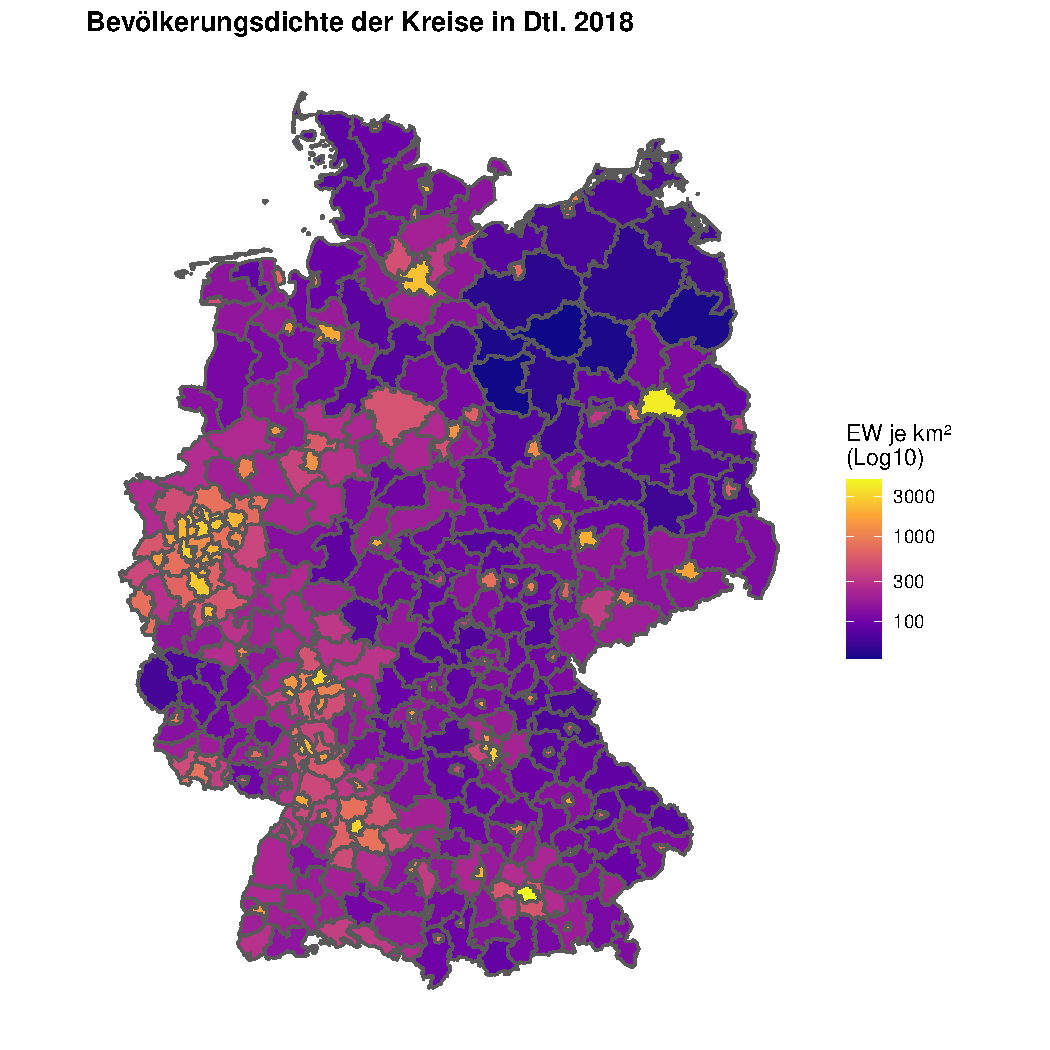
\includegraphics[width=\linewidth,trim={2cm 1cm 1cm 1cm},clip]{body/figures/popdens2018.pdf} % [scale=0.5] oder [width=\linewidth]
       %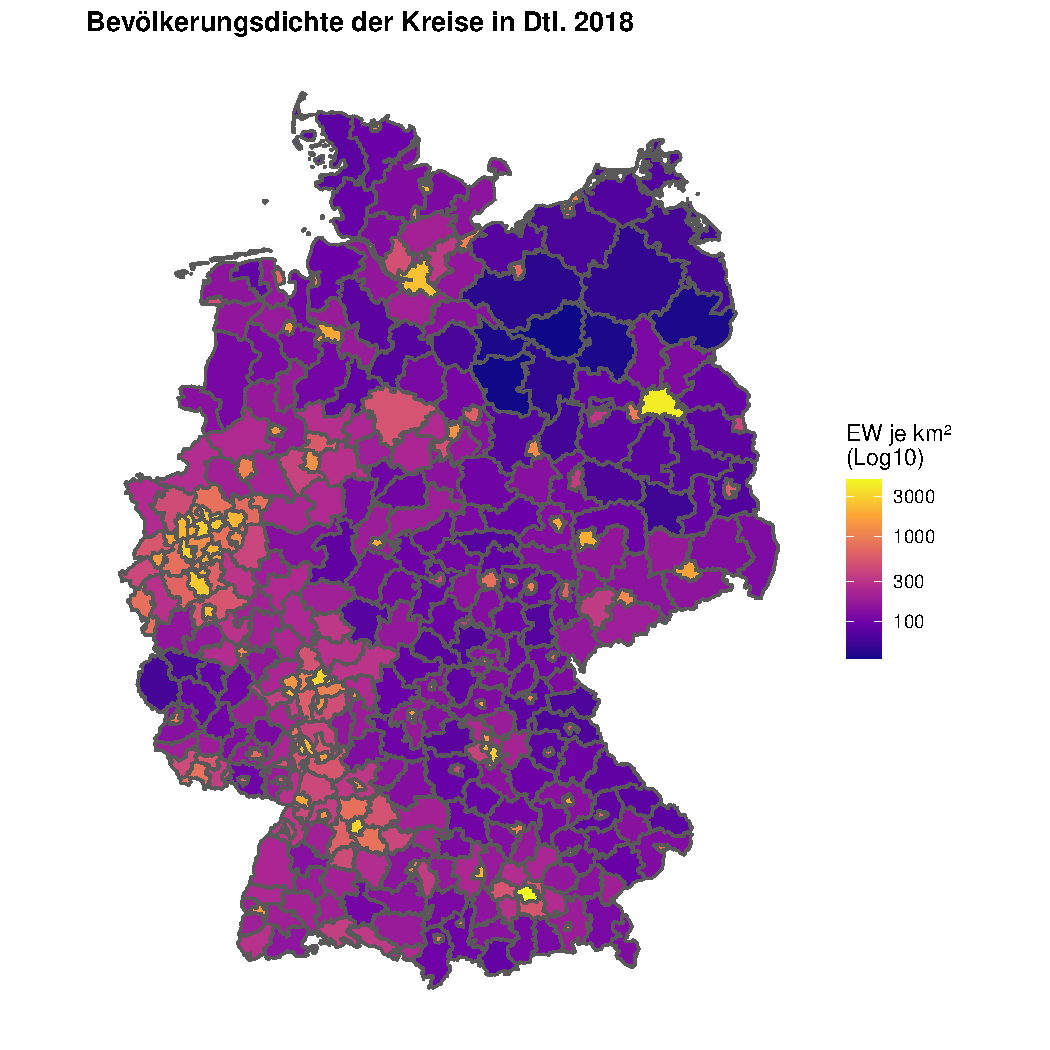
\includegraphics[scale=0.4,trim={1cm 2cm 1cm 2cm},clip]{body/figures/popdens2018.pdf} % [scale=0.5] oder [width=\linewidth]
       %[width=\textwidth] entspricht [width=\linewidth] (=Breite einer Minipage)
       \caption{reale Daten}
    \end{minipage} % <- sonst wird hier ein Leerzeichen eingefügt
    \hfill
    %\hspace{.1\linewidth}% Abstand zwischen Bilder
    \begin{minipage}[b]{.45\linewidth}
        %\centering
       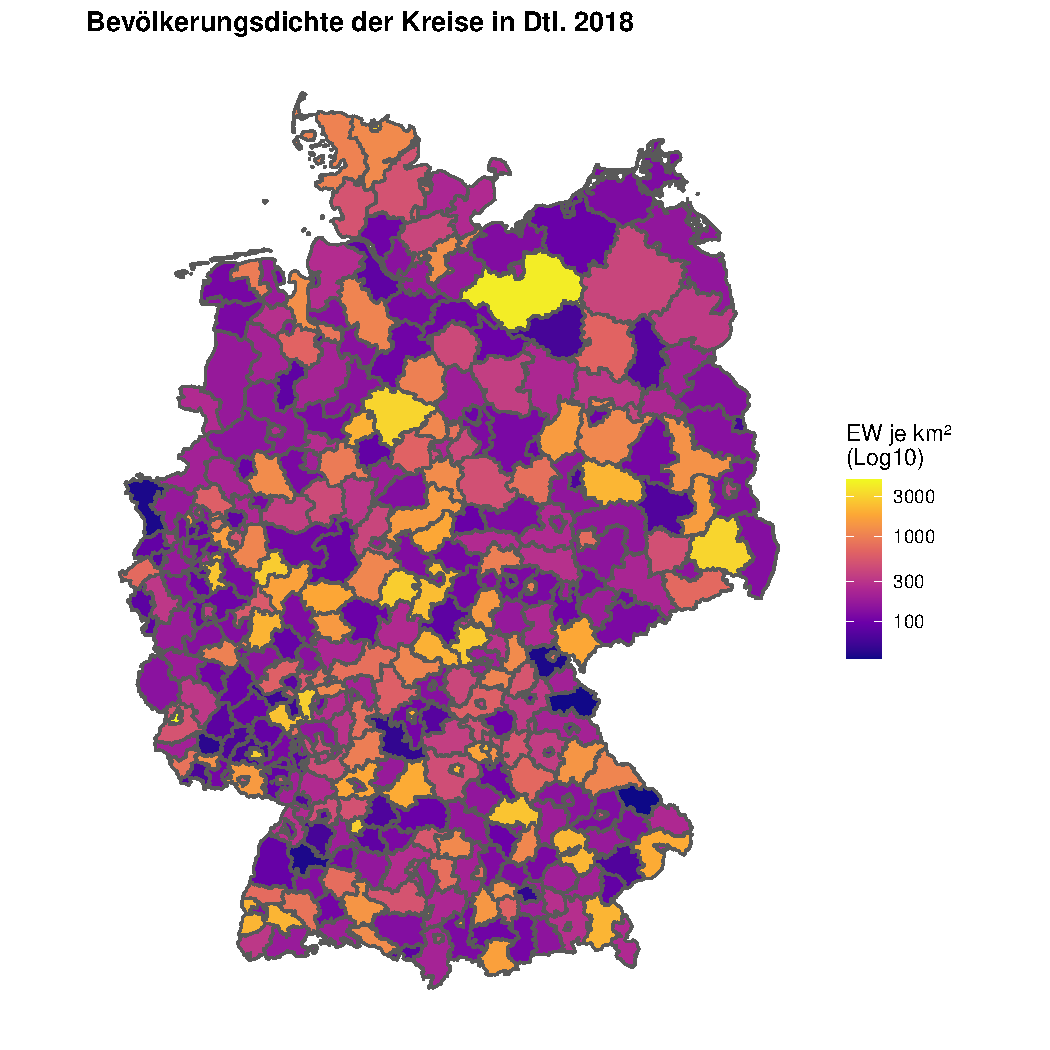
\includegraphics[width=\linewidth,trim={2cm 1cm 1cm 1cm},clip]{body/figures/popdens2018-rdm.pdf}
       \caption{randomisierte Daten}
    \end{minipage}
    \caption[Bevölkerungsdichten ]{Autokorrelation der Bevölkerungsdichte je Kreis in 2018. Grafik erstellt mit Daten aus: Quelle}
    \label{fig_densitymaps}
 \end{figure}

Hier besteht die Annahme, dass räumlich benachbarte Beobachtungen einer Variablen/Attributs ähnlicher 
sind als weit entfernte. Dieser Umstand wird durch Toblers erstes Gesetz der Geographie 
ausgedrückt \cite[S.234]{tobler_computer_1970}:
\begin{quotation}
    \glqq […] \textit{the first law of geography: everything is related to everything else, 
    but near things are more related than distant things.}\grqq{} Waldo R. Tobler
\end{quotation}
Trotz ihrer simplen Präsentation und obwohl diese Formulierung eher wie 
common sense anmuted und fraglich ist, ob tatsächlich 
\glqq alles miteinander in Beziehung steht\grqq{} wie \cite{tobler_first_2004} selbst anmerkt, 
so ist er der erste Wissenschaftler, der dieses grundlegende Konzept 
räumlicher Dynamik klar ausformulierte. \newline
Inwiefern zwischen einem universalen wissenschaftliches Gesetz und einer beobachteten 
Regelmäßigkeit (engl. causality vs regularity) unterschieden werden kann und ob in 
den Sozialwissenschaften von Gesetzen gesprochen werden kann, ist Gegenstand 
wissenschaftlicher Auseinandersetzung (e.g. Law of Utility Maximization) \cite{goodchild_validity_2004}. 
Tobler argumentiert mit der Distanz als Ursache und argumentiert somit gegen die Sicht, 
dass Distanz und räumliche Verteilung von Merkmalen als zwei Beobachtungen einer 
verborgenen Ursache nur „beobachtete Regelmäßigkeiten“ sind. (Verweis auf Feynman?) \cite{sui_toblers_2004} 
%Block eher in die Einleitung?
Die Theorie fällt historisch in die Zeit der Quantitativen Revolution der 
modernen Geographie (s. Kapitel1?), wird jedoch erst mit Aufkommen und Verbreitung 
geographischer Informationssysteme (GIS) seit den 1990er Jahren in größerem Umfang 
beachtet, gelehrt und referenziert [Sui-Forum].
%Ende

Das Gesetz entspricht der menschlichen Intuition aus historischen 
Beobachtungen und ist fest verankert in wissenschaftlichen Paradigmen. 
In der Theorie basiert diese Gesetzmäßigkeit wiederum auf dem Konzept 
der \emph{Distanzreibung} (engl. friction of distance) 
und daraus resultierenden Abklingfunktionen (engl. distance decay) für allgemeine räumliche Merkmale. 
Derartige Abklingfunktionen bilden die Grundlage für die Interpolationsmethoden der \emph{Geostatistik}, 
wie in Kapitel \ref{subsec:geostatistics} näher erläutert wird.
Weitere Grundlage räumlicher Interpolation ist die Messung der Ähnlichkeit räumlich benachbarter Merkmale 
als Ziel der Theorie \emph{räumlicher Autokorrelation} (engl. spatial autocorrelation). 
%Abschnitt in Autokorrelationskapitel rein
Die räumliche Lage/Position einer Punktmessung liefert selbst bereits implizit inhärente Zusatzinformationen 
über die Beobachtungswerte in der Umgebung des Beobachtungswertes. 
Diese Autokorrelation stört somit die Grundannahme einer \emph{unabhängig identisch verteilten} (i.i.d.) Grundgesamtheit, 
da Messungen an verschiedenen Positionen nicht unabhängig voneinander sind, insbesondere bei geringer Distanz zueinander. 
%Abschnitt-Ende
In Kapitel \ref{ch:autocorrelation} werden globale und lokale Autokorrelationsindikatoren zur 
Detektion räumlich-zeitlicher hot- und coldspots und als Werkzeuge der Regression eingeführt.

Zunehmende Distanz erhöht zudem die Kosten der Interaktion zwischen Raumpunkten. 
Im Beispiel der sozio-ökonimschen Gravitationsmodelle beeinflussen 
der (teilweise in Transportkosten enthaltene) Energie-, Zeit und Materialaufwand für Mobilität  
die kulturelle, soziale und politisch-wirtschaftliche Distanz.
Die Distanzreibung dient zudem der Erklärung historischer Wirtschaftsentwicklung, 
militärischer Dominanz eines Staates 
bis hin zu ökologischen Ausbreitungsmustern von Vegetationszonen und Tierarten. 
Das geografische Gesetz begründet auf Grundlage dieser Distanzeffekte die Beobachtung annähernd 
homogener Regionen und zusammenhängende Gebiete mit 
ähnlichen Merkmalen (e.g. Städte, Vegetationszonen, Planetensysteme? Usw.).

Geringere Bekanntheit erlangte Toblers zweites Gesetz: 
\glqq\textit{The phenomenon external to an area 
of interest affects what goes on inside}\grqq{}.
Hiermit weist er darauf hin, dass in praktischen Experimenten die Abmessungen des endlichen 
Beobachtungsraumes zu einem bestimmten Grad willkürlich gewählt sind und weiterhin durch Vorgänge über 
die Abgrenzung hinaus beeinflusst werden. 
Viele Phänomen weisen Autokorrelationen zwischen räumlichen Zonen auf, (welche nicht im untersuchten Prozess begründet liegt?).
Problematisch ist die fehlende Unabhängigkeit der Stichproben aufgrund der räumlichen Nähe. 
Eine Auseinandersetzung ist 1889 als "Galtons Problem" überliefert, in welcher Sir Francis Galton auf Fehlschlüsse hinweist, sobald Daten nicht mehr unabhängig voneinander sind.
Er zeigte, dass positive räumliche Abhängigkeit den Informationsgehalt der Beobachtungen verringert, 
da sie durch andere Beobachtungen in der Nähe teilweise prognostiziert werden können. 
Dies reduziert den effektiven Stichprobenumfang. In solch einem Fall liegt den abhängigen Daten ein gemeinsamer Vorgang zugrunde, 
während eine räumliche Aufteilung in verschiedene Zonen voneinander unabhängige Daten suggeriert/vorgaukelt (Bivand S. 264).

Im folgenden Abschnitt wird auf weitere Probleme der Zerlegung und Skalierung eingegangen.

\subsection*{Räumliche Aggregationseffekte}
Beobachtungsmerkmale können durch Skalierung ihr Verhalten/Gesetzmäßigkeiten ändern. 
So lässt sich die Länge einer Küstenlinie nicht eindeutig bestimmen, sondern wird aufgrund ihrer 
fraktalen(?) Struktur mit abnehmender Meßstablänge in zunehmender Länge gemessen, 
ohne gegen einen endlichen Wert zu konvergieren. 
Daher wird nach Möglichkeit auf skaleninvariante Messgrößen zurückgegriffen.
(Beispiele für dimensionslose Größen sind normalisierte Standardverteilungen und ihre Momente sowie 
entparametrisierte Pivotzufallsgrößen. Auch ein Wiener Prozess ist skaleninvariant.)

Darüber hinaus treten Aggregationseffekte bei Änderungen der räumlichen Auflösung sowie Vergleichen/Beziehungen über/zwischen verschiedene Maßstäbe auf.
Dieses Problem ist als \emph{Problem des Trägerwechsel?/veränderlicher Bezugsregion}(engl. change-of-support problem - COSP) bekannt und 
wurde durch Cressie (1996) formalisiert. Der räumliche Träger bezeichnet hierbei Form, Größe und Orientierung der Messeinheiten, 
abstrakt beschrieben durch Punkte, Linien oder Flächen/Gebiete als Merkmale (engl. features) des Raumes. 
Eine Änderung der Merkmale des Trägers einer Variablen, etwa durch Aggregation, erzeugt/definiert eine neuartige Variable mit neuen/abweichenden statistischen und räumlichen Eigenschaften.
Die Beziehung der räumlichen Variation beider Variablen ist der Kern des COSP. (Waller Gotway S.107)
Das Problem manifestiert sich durch Instabilität statistischer Resultate bei Änderung der Aggregationsweise. 
Zum Beispiel ließe sich Bevölkerungseinkommen als räumliche Variabe über dem Träger der punktgenauen Wohnadressen erfassen und ihre Variation betrachten.
Eine Aggregation der Daten in Stadtviertel als weiteren möglichen Träger resultiert in einer anderen Variation der Einkommensvariablen.


Das Problem tritt für unterschiedliche Anwendungen in vielfältigen Varianten auf.  
Auf dem Gebiet der \emph{Geostatistik} sind Bohrkernproben im Gestein nur punktweise praktisch möglich (und einige cm³ groß), 
wodurch von einer Stichprobe an Bohrungen auf die Grundverteilung von Mineralien und Erzadern (mit vielen m³ Volumen) inter- und extrapoliert werden muss. 
In der Interpolation sind begrenzte Rohdaten in einer feinen Auflösung lückenhaft vorhanden und Inferenz wird in einer gröberen Auflösung (Umgebung der Bohrungen), 
über weiteren Lokationen oder Zonen benötigt.

% Das Format sogenannter \emph{Gitterdaten} wird im folgenden Abschnitt behandelt und am Beispiel der Bundesländer
Als Spezialfall des COSP für \emph{Gitterdaten} (KapitelXX) addressiert das \emph{Problem der veränderbaren Gebietseinheit} (engl. modifiable areal unit problem - MAUP)
die Aggregation von punktbasierten, kontinuierlichen Messgrößen (regionalisierten Variablen) über diskrete Raumzonen als zusätzliche Fehlerquelle. 
Abbildung \ref{fig_zoning} stellt Aggregationseffekte einer einfachen Zählvariablen schematisch dar.

\begin{figure}[htb] %h=here, t=top, b=bottom, p=page of float
    \centering %Bilder mittig statt am linken Rand ausgerichtet
    \begin{minipage}[b]{.32\linewidth} % [b] => Ausrichtung an \caption --> c (=Center) t (=Top) und b (=Bottom)
        % \linewidth entspricht hier \textwidth (=Breite Textbereich)
        %\centering
        %                                 trim = links unten rechts oben
        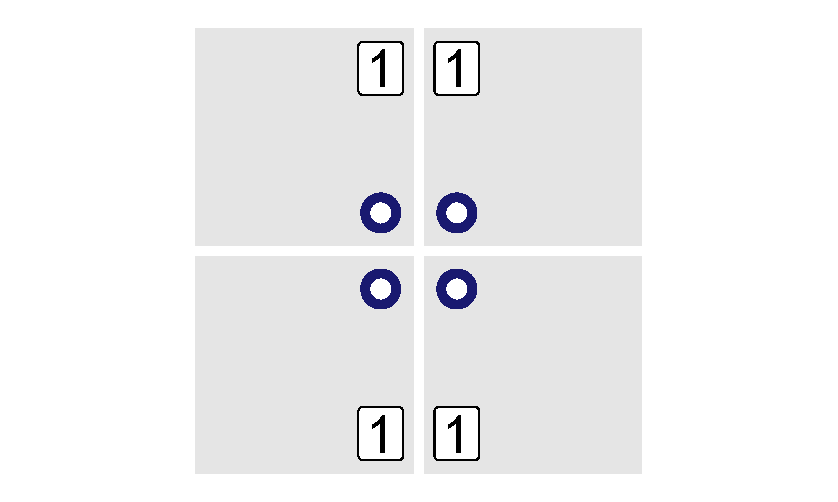
\includegraphics[width=\linewidth,trim={0.5cm 0.5cm 0.5cm 0.5cm},clip]{body/figures/41-maup_1.pdf} % [scale=0.5] oder [width=\linewidth]
       %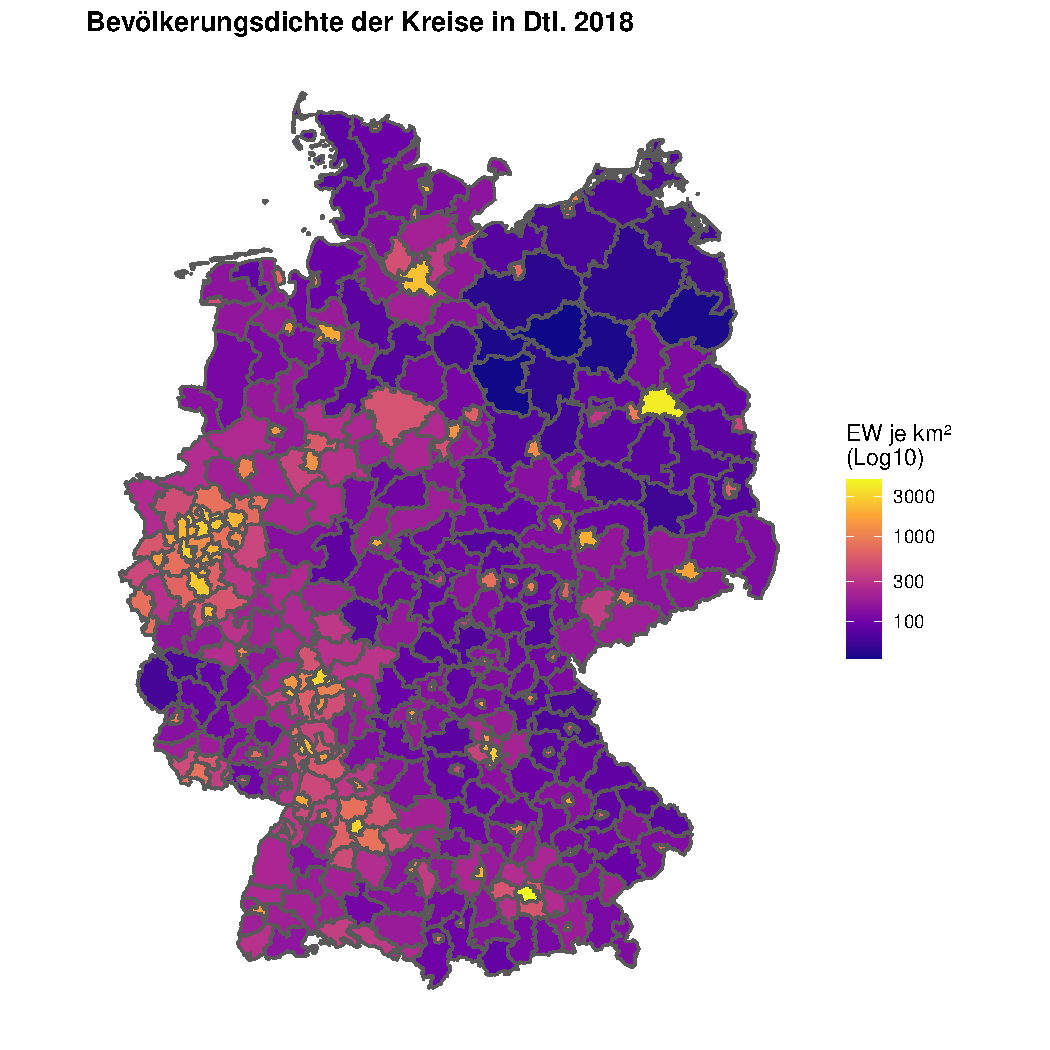
\includegraphics[scale=0.4,trim={1cm 2cm 1cm 2cm},clip]{body/figures/popdens2018.pdf} % [scale=0.5] oder [width=\linewidth]
       %[width=\textwidth] entspricht [width=\linewidth] (=Breite einer Minipage)
       %\caption{erste Nachbarn}
    \end{minipage} % <- sonst wird hier ein Leerzeichen eingefügt
    \hfill
    %\hspace{.1\linewidth}% Abstand zwischen Bilder
    \begin{minipage}[b]{.32\linewidth}
        %\centering
       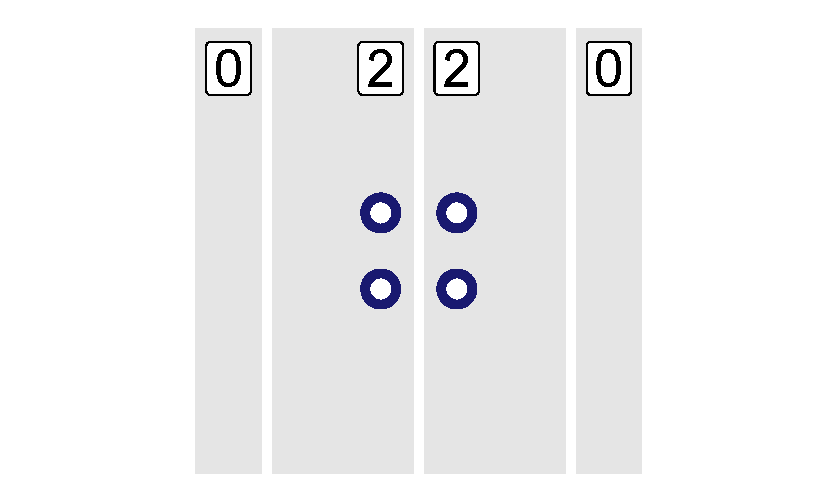
\includegraphics[width=\linewidth,trim={0.5cm 0.5cm 0.5cm 0.5cm},clip]{body/figures/42-maup_2.pdf}
       %\caption{zweite Nachbarn}
    \end{minipage}
    \hfill
    %\hspace{.1\linewidth}% Abstand zwischen Bilder
    \begin{minipage}[b]{.32\linewidth}
        %\centering
       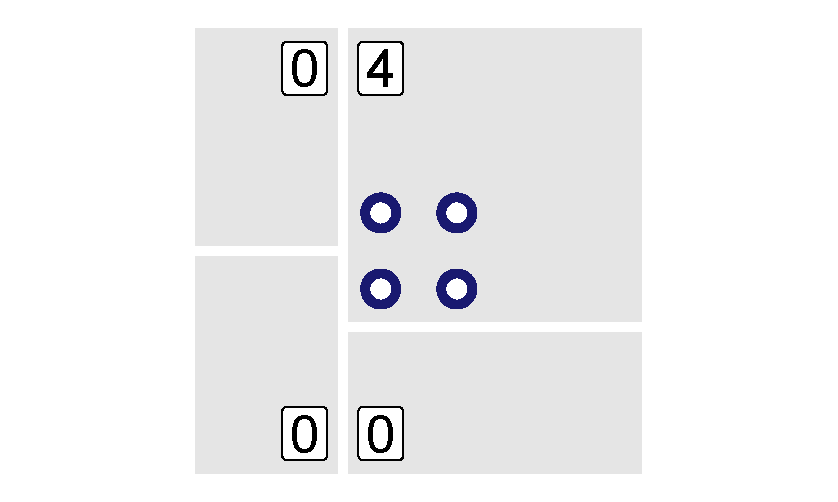
\includegraphics[width=\linewidth,trim={0.5cm 0.5cm 0.5cm 0.5cm},clip]{body/figures/43-maup_3.pdf}
       %\caption{zweite Nachbarn}
    \end{minipage}
    \caption[Zoneneffekt]{Einfacher Zoneneffekt für 3 Konfigurationen von 4 Zonen }
    \label{fig_zoning}
 \end{figure}

Dies betrifft beispielsweise die Angabe von Bevölkerungsdaten, welche zwar theoretisch punkteweise an adressgenauen Lokationen oder GPS-Raumpunkten erfasst werden können, 
aber aus Datenschutzerwägungen oder aufgrund der Verwaltungsmethodik ohne genaue Adresse erfasst werden und stattdessen auf Gemeindeebene zusammengefasst sind. 
Viele geografische Rohdaten sind nur als derartige Zähldaten/Raten per Raumeinheit bzw. Zone verfügbar. 
Diese sind typischerweise willkürlich, zeitlich veränderlich und haben oft keine intrinsische geografische Bedeutung (Fischer,Getis 2009- Handbook S.213).
(Auch die Dichte der Population je Fläche ist theoretisch messbar in $\epsilon$-Umgebung von punktgenauen, (stetigen) Raumpunkten.) 
Praktisch aber wie die Rohdaten auf Zonen verdichtet, erlaubt sie zumindest den Vergleich verschieden großer Zonen.
Aggregiert (z.b. Mittelwertbildung) werden diese über Verwaltungszonen wie etwa Bundesländer.  
% Die Bevölkerungswerte beliebiger Raumpunkte auf einer nach Bundsländern aufgeteilten Karte lassen durch Modifikation der Aggregation nach Gemeinden abändern. 

Dem Aggregationsproblem liegt im Detail das Zusammenspiel zweier zusammenhängender Effekte zugrunde. 
Zum einen kann eine feste Stichprobe über unterschiedlich feine Partitionen der Gebietsflächen verdichtet werden. 
Daraus resultiert ein Vergleich von Daten unter verschiedenen räumlichen Auflösungen (engl. spatial resolution) bzw. Maßstäben (engl. spatial scale)
und wird als \emph{Skalierungseffekt} (engl. scale or aggregation effect) bezeichnet.
Dies beinhaltet auch das Problem unterschiedlicher Granularität innerhalb einer Auflösungsstufe. 
So stehen etwa einige großflächige (dünnbesiedelte) Gemeinden im direkten Vergleich mit sehr kleinen (dichtbesiedelten) Gemeinden.
Werden hingegen bei fester/gegebener Auflösung mit konstanter Anzahl der Raumeinheiten einzelne Grenzverläufe verschoben und Gebietseinheiten so zu einer neuen Konfiguration verformt, 
so werden resultierende Inkonsistenzen räumlicher Variation und Ergebnisschwankungen der Inferenz als \emph{Zoneneffekt} (engl. grouping or zoning effect) bezeichnet. 
Theoretisch wäre eine Situation denkbar, in der (per Volksentscheid) ein Bundesland/Distrikt/Land Teilgebiete an ein anderes übergibt 
oder für eine feste Anzahl Verwaltungszonen neue Abgrenzungen/Grenzverläufe definiert werden.
Abbildung \ref{fig_zoning2} gibt schematisch den Zoneneffekt einer räumlichen Variable bei Mittelwertbildung wieder.

\begin{figure}[htb] %h=here, t=top, b=bottom, p=page of float
    \centering %Bilder mittig statt am linken Rand ausgerichtet
    \begin{minipage}[b]{.32\linewidth} % [b] => Ausrichtung an \caption --> c (=Center) t (=Top) und b (=Bottom)
        % \linewidth entspricht hier \textwidth (=Breite Textbereich)
        %\centering
        %                                 trim = links unten rechts oben
        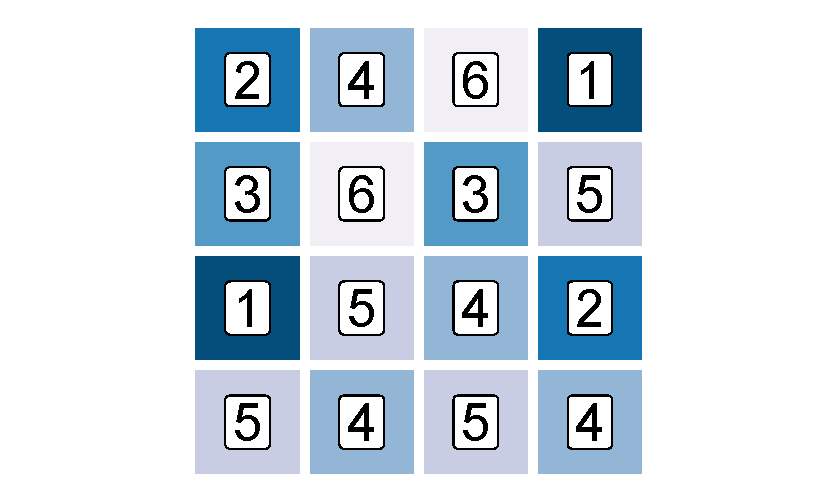
\includegraphics[width=\linewidth,trim={0.5cm 0.5cm 0.5cm 0.5cm},clip]{body/figures/44-zon_a.pdf} % [scale=0.5] oder [width=\linewidth]
       %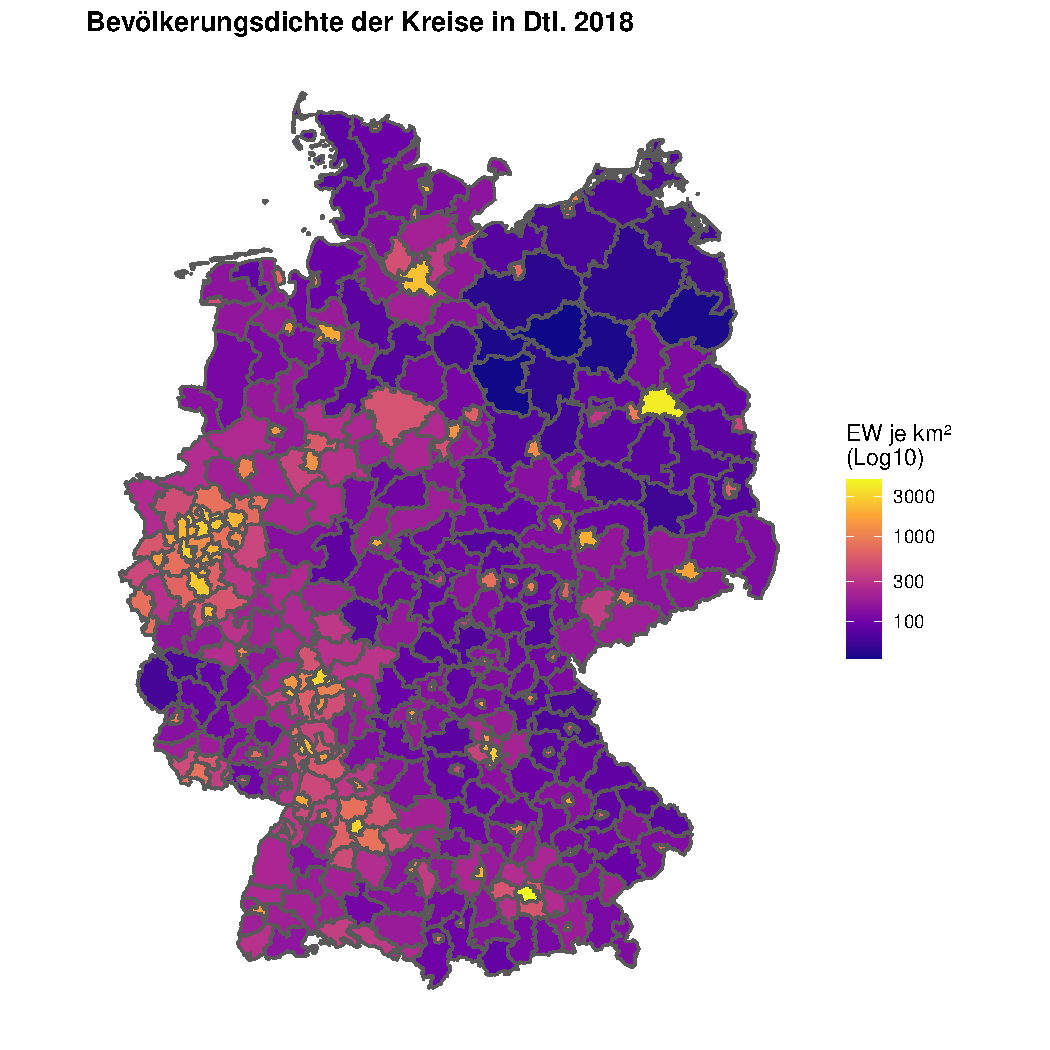
\includegraphics[scale=0.4,trim={1cm 2cm 1cm 2cm},clip]{body/figures/popdens2018.pdf} % [scale=0.5] oder [width=\linewidth]
       %[width=\textwidth] entspricht [width=\linewidth] (=Breite einer Minipage)
       %\caption{erste Nachbarn}
    \end{minipage} % <- sonst wird hier ein Leerzeichen eingefügt
    \hfill
    %\hspace{.1\linewidth}% Abstand zwischen Bilder
    \begin{minipage}[b]{.32\linewidth}
        %\centering
       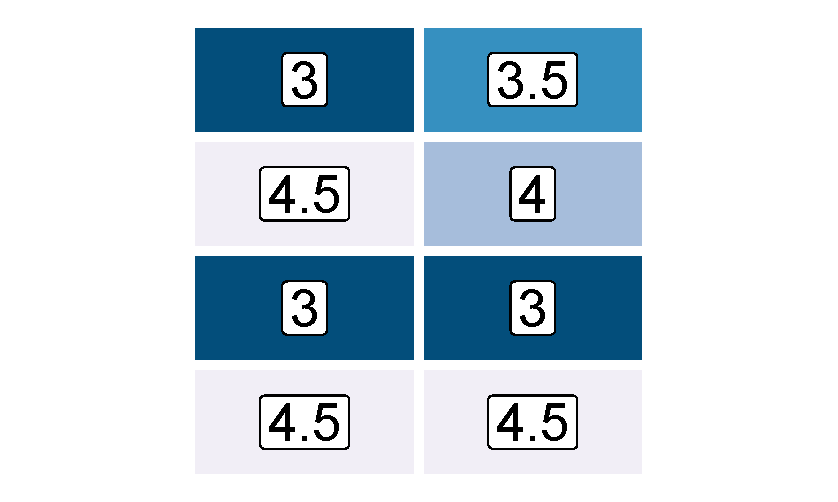
\includegraphics[width=\linewidth,trim={0.5cm 0.5cm 0.5cm 0.5cm},clip]{body/figures/45-zon_b.pdf}
       %\caption{zweite Nachbarn}
    \end{minipage}
    \hfill
    %\hspace{.1\linewidth}% Abstand zwischen Bilder
    \begin{minipage}[b]{.32\linewidth}
        %\centering
       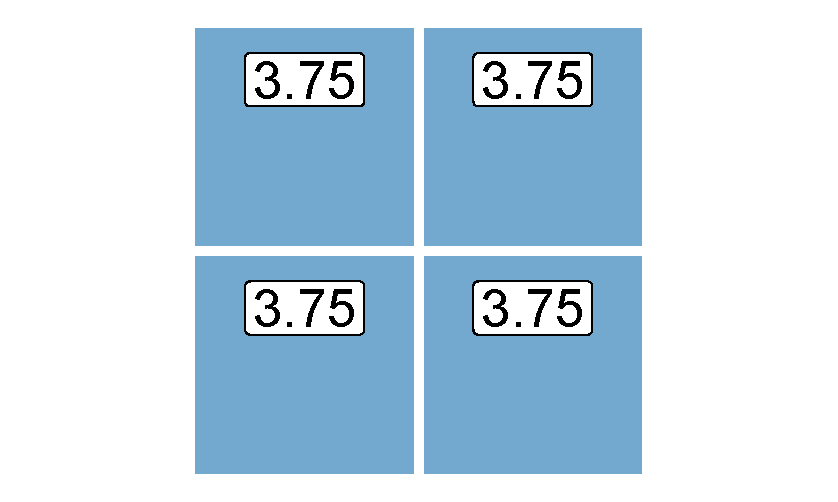
\includegraphics[width=\linewidth,trim={0.5cm 0.5cm 0.5cm 0.5cm},clip]{body/figures/46-zon_c.pdf}
       %\caption{zweite Nachbarn}
    \end{minipage}
    \caption[Zoneneffekt]{Zonneneffekt für 3 (bzw. 2) Konfigurationen von 4 (bzw. 8) Zonen }
    \label{fig_zoning2}
 \end{figure}

Weiterhin gibt es:

\begin{figure}[htb] %h=here, t=top, b=bottom, p=page of float
    \centering %Bilder mittig statt am linken Rand ausgerichtet
    \begin{minipage}[b]{.32\linewidth} % [b] => Ausrichtung an \caption --> c (=Center) t (=Top) und b (=Bottom)
        % \linewidth entspricht hier \textwidth (=Breite Textbereich)
        %\centering
        %                                 trim = links unten rechts oben
        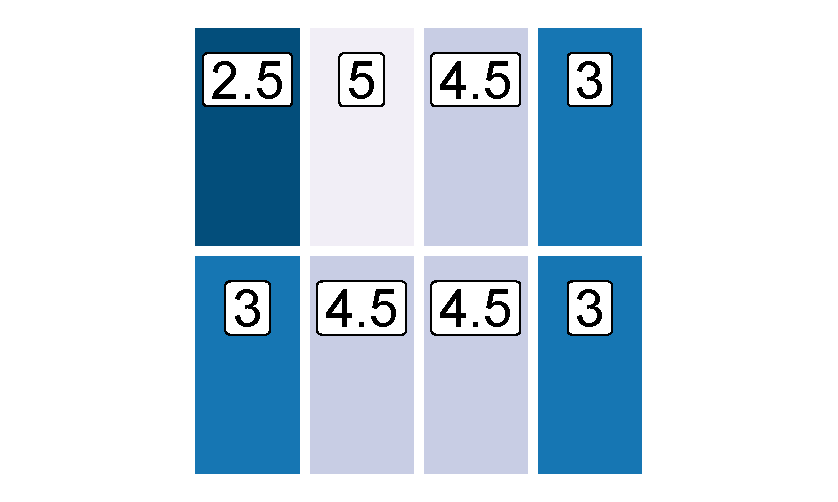
\includegraphics[width=\linewidth,trim={0.5cm 0.5cm 0.5cm 0.5cm},clip]{body/figures/47-zon_d.pdf} % [scale=0.5] oder [width=\linewidth]
       %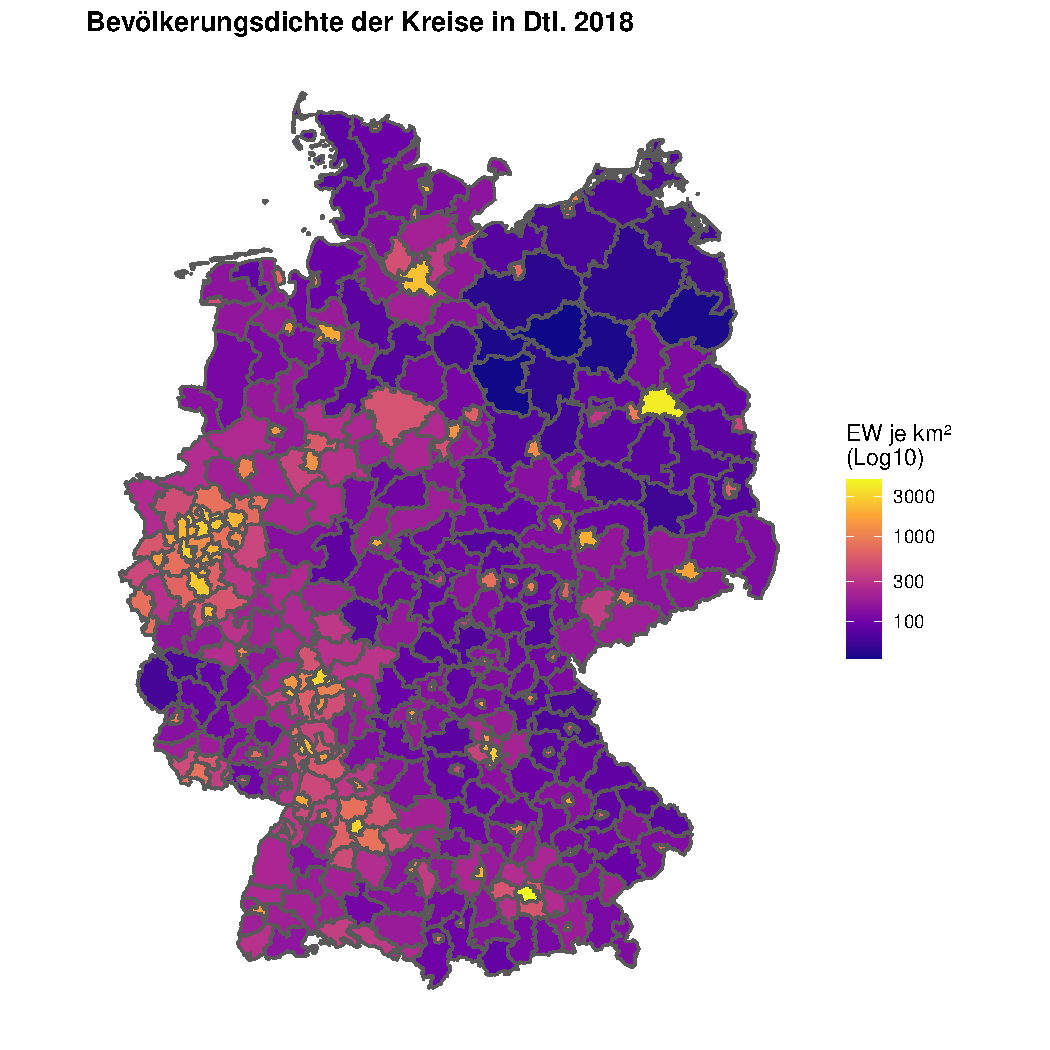
\includegraphics[scale=0.4,trim={1cm 2cm 1cm 2cm},clip]{body/figures/popdens2018.pdf} % [scale=0.5] oder [width=\linewidth]
       %[width=\textwidth] entspricht [width=\linewidth] (=Breite einer Minipage)
       %\caption{erste Nachbarn}
    \end{minipage} % <- sonst wird hier ein Leerzeichen eingefügt
    \hfill
    %\hspace{.1\linewidth}% Abstand zwischen Bilder
    \begin{minipage}[b]{.32\linewidth}
        %\centering
       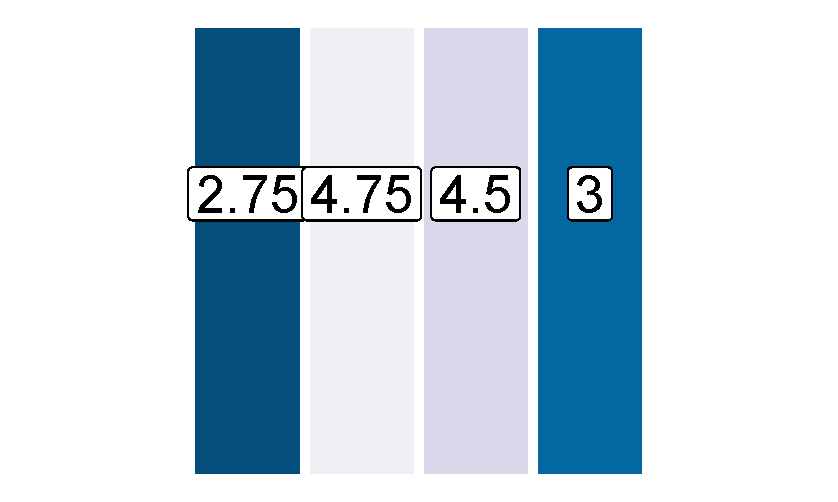
\includegraphics[width=\linewidth,trim={0.5cm 0.5cm 0.5cm 0.5cm},clip]{body/figures/48-zon_e.pdf}
       %\caption{zweite Nachbarn}
    \end{minipage}
    \hfill
    %\hspace{.1\linewidth}% Abstand zwischen Bilder
    \begin{minipage}[b]{.32\linewidth}
        %\centering
       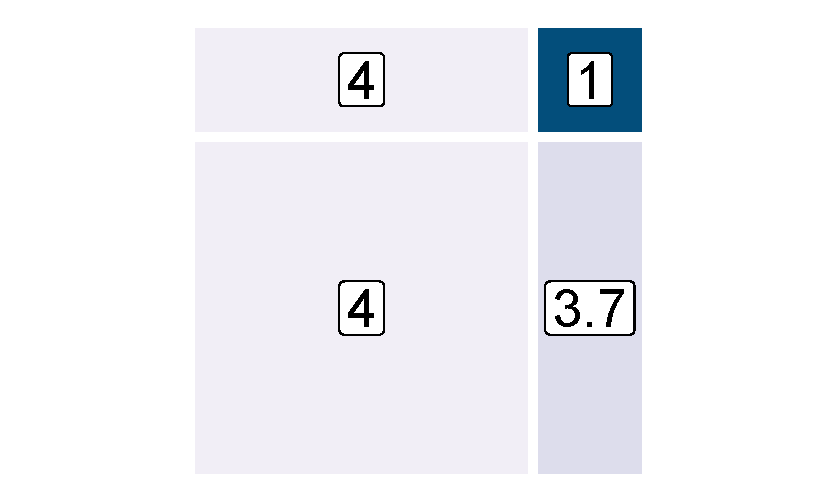
\includegraphics[width=\linewidth,trim={0.5cm 0.5cm 0.5cm 0.5cm},clip]{body/figures/49-zon_f.pdf}
       %\caption{zweite Nachbarn}
    \end{minipage}
    \caption[Zoneneffekt]{Zonneneffekt für 5 Konfigurationen von 4 Zonen }
    \label{fig_zoning3}
 \end{figure}

Ein Datensatz kann somit durch unterschiedliche Aggregationskonfigurationen verschiedene Ergebnisse erzeugen. %doppelt?
Dieser Effekt kann Fehler und Missinterpretationen verursachen, wird aber auch zur bewussten Manipulation eingesetzt. 
In der politischen Festlegung von Wahldistrikten sind insbesondere in den USA das \emph{gerrymandering} und \emph{political redistricting} als Wahlbeinflussung hochumstritten.
Aber auch in unserem vorliegenden Forschungsprojekt sind die (willkürlichen) Gemeindeverläufe kritisch zu beachten. Die Analyse wird verzerrt, sobald der zugrundeliegende, datengenerierende
Prozess nicht ausreichend exakt durch die Partition gedeckt ist und übereinstimmt. 
Eine Miskonfiguration/Fehlspezifizierung des Modells erzeugt bereits eine räumliche "Schein"-autokorrelation. 
Andererseits können auch räumliche Muster/Informationen in den Residuen verschwinden.
Verwaltungsgrenzen sind oft willkürlich gesetzt und ändern sich im Zeitverlauf. %DOPPELT
Auch wenn diese Grenzen ex-ante vorgegeben sind, so weist dieser Bias auf die direkte Abhängigkeit der Ergebnisse vom Aggregationsvorgang hin. 
Weitere Zerlegungsprobleme werden in Kapitel XX aufgezeigt. 
Die exakte Untersuchung von räumlichen Mustern und Kenngrößen wird durch derartige Aggregation behindert. Im Gegensatz zu systematischer Informationsverdichtung nach 
statistischer Methodik welche (für sinnvolle Kennzahlanalyse?) notwendig ist, handelt es sich um inkonsistente Rohdatensätze bereits zu Analysebeginn. (Anselin and Getis, 1992?). 

Zugleich muss in der Analyse zwischen verschiedenen Aggregationsstufen transformiert werden 
(data downscaling - data disaggregation und data upscaling via integration/aggregation reduces spatial heterogeneity ).
upscaling’ (aggregation) and ‘downscaling’ (disaggregation).

Das Problem setzt sich in der statistischen Inferenz fort, (da Korrelation von den Varianzen abhängt?.). 
Die Problematik geht aber weit über Varianzen und Korrelationen hinaus und betreffen Regressionen, hierarchische Methoden und weitere räumlich statistische Methoden (Waller Gotway, S.106).
Werden statistische Kennzahlen über eine bestimmte Konfiguration von Distrikten/Zonen gebildet (gemittelt/aggregiert), 
so stimmen aus dieser Zusammenfassung gezogene Schlüsse/Inferenzen nicht notwendig überein mit den Schlüssen, die eine andere Konfiguration der Distrikte liefert.
Besonders bei der Ableitung von individuellen Kennzahlen (Risikokenngrößen usw) für einzelne Individuen aus regionalen/lokalen Gebietsdaten muss mit Vorsicht agiert werden. 
Auch wenn die Verhältnisse/Maße/Anteile gebietsübergreifend stabil sind und die Populationen ähnlich groß eingeteilt sind. (Waller Gotway, S.104 - schwache Ref..)

Der Begriff wurde durch Openshaw and Taylor (1979) geprägt, indem sie systematisch demonstrierten, 
wie sehr Korrelationskoeffizienten für einen festen Datensatz variieren können, indem nur die Raumpartition manipuliert wird.
Über das zugrundeliegende Problem instabiler Inferenz wird jedoch bereits seit den 1930er Jahren publiziert (Gehlke and Biehl 1934).

Monmonier (1996 S.218 ff.) illustriert derartige Probleme/Effekte am berühmten Beispiel der Londoner Cholera-Karte des Mediziners John Snow aus dem Jahre 1856?, deren
historische Bedeutung in Kapitel \ref{sec:generalmodel} noch deutlich wird.
% Die punktgenauen Adressen von Choleratoten werden über 3 verschiedene Konfigurationen von Distrikten aggregiert und liefern widersprüchliche Aussagen.
% Die ursprünglich erkennbaren Cluster werden verwässert ( Verwischen der Clusterpunkte?).

Making statistical inferences about individuals based on aggregate data is flawed.

Das MAUP ist die geografische Manifestation des \emph{Ökologischen bzw. Kollektiven Fehlschluss/Bias} (engl. ecological inference problem or fallacy), 
1950 vom Statistiker William S. Robinson formuliert. 
Dies bezeichnet den fehlerhaften Vergleich von Individuen verschiedener Gruppen auf Basis von Kenngrößen auf Gruppenlevel statt der gesamten Verteilungen der Messgrößen.

% King (1997, p.252)
the MAUP is not an empirical problem. If we want statistics that are invariant to the level of aggregation then we should not use regression or correlation, but use
statistics that are invariant (see also Tobler 1990).

Die Lösungsansätze sind sehr spezifisch auf Einzelfälle anwendbar ohne Generalisierungen. 
Openshaw (1984) concluded that it is unlikely that an analytical solution to the MAUP will ever be realized due to the wide range of possibilities 
that arise when the partitioning of continuous space is implemented as well as the wide range of analytical tasks that aggregated data are required to perform (see also Wong 2009). 

%(Gotway CA &Young LJ 2002) - Combining incompatible spatial data.
% solutions to the COSP including geostatistical solutions based on different forms of kriging and map overlay solutions (point in polygon, areal weighting, spatial smoothing and regression methods).
% also review multiscale modeling solutions (multiscale spatial tree models and Bayesian hierarchical models).
% the common solution strategy for COSP is to build a model from data with small support and use that to estimate parameters and make valid inferences.

%Dray et. al 2012 - Community ecology in the age of multivariate multiscale spatial analysis
%mismatches are among the reasons for finding spatial autocorrelation in analysing areal aggregates;
%other reasons include substantive spatial processes in which entities influence each other by contagion, such as the adoption of similar policies by neighbours,
%and model misspecification leaving spatially patterned information in the model residuals.

FÜr eine gute Übersicht siehe \cite[S.104]{waller_applied_2004} und Haining S. 
Für umfangreiche und tiefergehende Details siehe Fischer Handbook 2014 Kapitel 59, S.1157-1169
sowie Gelfand et al. Handbook Kapitel 29, S.517-536 
Probleme für Ökonometrie: Cressie 1998, Arbia,Petrarca
% N. A. Cressie (1998). Aggregation and interaction issues in statistical modeling of spatiotemporal processes. Geoderma
% Arbia-Effects of MAUP on spatial econometric models


% Gehlke, C. E.; Biehl, Katherine (March 1934). "Certain effects of grouping upon the size of the correlation coefficient 
%           in census tract material". Journal of the American Statistical Association. 29 (185A): 169–170. doi:10.2307/2277827.
% Yule, Kendall (1950).  p. 312
% McCarthy 1956
% S. Openshaw and P. J. Taylor (1979). A million or so correlation coefficients: three experiments on the modifiable areal unit problem.Statisticalapplications in the spatial sciences, 21:127–144
% Openshaw, S. (1984). The Modifiable Areal Unit Problem. CATMOG 38. Norwich: Geo Books. ISBN 0-86094-134-5
% N. A. Cressie (1996). Change of support and the modifiable areal unit problem.Geographical Systems, 3:159–180
% 

% Manley, D. (2014). Scale, aggregation, and the modifiable areal unit problem. 
% In M. M. Fischer & P. Nijkamp (Eds.), Handbook of regional science (pp. 1157–1171). Berlin: Springer-Verlag.

\section{Allgemeines Modell räumlicher Stochastik}
\label{sec:generalmodel}

Die Grundkomponenten der mehrdimensionalen Lageanalyse sind räumlich verteilte Positionen 
$\left\{ s_1 , s_2 ,\ldots , s_n \right\}$ mit an diesen Positionen beobachtete 
Daten $\left\{ Z(s_1),Z(s_2),\ldots,Z(s_n) \right\}$ als Realisierungen des Attributes Z. 
Sowohl stetige (metrisch) als auch diskrete (ordinal- oder nominalskalierte) Daten sind 
an regulär oder irregulär angeordneten Positionen in einem stetigen oder diskreten Raum möglich. 
Das Standardwerk(?) von Cressie p.8 liefert eine flexible theoretische Struktur. \\

Sei $s \in \RR^d \mathds{R}^d $ eine unspezifische (generische/anwendungsneutrale) Position 
im $d$-dimensionalen euklidischen Raum 
und $Z(s)$ eine Zufallsgröße (eines Datums?) an Position $s$. 
Unter Variation von $s$ über Indexmenge bzw. Definitionsbereich (engl. domain) $D \subseteq \RR^d$ 
wird der stochastische Prozess 
\begin{equation*}
    \left\{ Z(s):s \in D \right\}
\end{equation*}
als multivariates Zufallsfeld (bzw. Zufallsprozess) beschrieben.

Liegt der Fokus auf einer festen, endlichen Menge räumlicher 
Positionen $ \left\{  s_1 , s_2 ,\ldots , s_n \right\} \subseteq \RR^d$, 
dann ist $ \left( Z(s_1),Z(s_2),\ldots,Z(s_n) \right)^{\top} $ ein Zufallsvektor, 
dessen multivariate Verteilung die räumlichen Abhängigkeiten der Beobachtungsvariable $Z$ widerspiegelt. 
Eine Realisierung dieses Zufallsfeldes wird mit $\left\{ z(s):s \in D \right\}$ ausgedrückt.

Eine nützliche Unterteilung von praktisch konstruierbaren Prozessen in 3 Hauptklassen 
wird durch \cite{cressie_statistics_1993} gegeben und in 
Tabelle \ref{table_main-classes} zusammengefasst. 
Diese Einteilung orientiert sich an der historischen 
Entwicklung in Abhängigkeit verschiedener Untersuchungsobjekte und unterscheidet bezüglich 
der Modellierung und ihrer Dimensionen.

\begin{table}[h!]
    \begin{center}
    \begin{tabular}{|r|c|c|}
    \hline
            & \multicolumn{2}{|c|}{\sc Position - unabhängig, exogen} \\
            \cline{2-3}
            & {\sc diskrete Variation}  & {\sc stetige Variation} \\
    \hline
    \multirow{3}{*}{\sc kein Attribut}  &    \multirow{3}{*}{-}    & \textbf{Punktprozesse} \\
            &                   & Krankheitsausbreitungen \\
            &                   & (ab ca. 1960) \\
    \hline
    \multirow{2}{*}{\sc Attribut -} & \textbf{Gitterdaten} & \textbf{Geostatistik} \\    
              & Ertrag der Landwirtschaft & Verteilung Bodenschätze \\
    {\sc abhängig, endogen}   & (ab ca. 1910) & (ab ca. 1970) \\
    \hline
    \end{tabular}
    \end{center}
    \caption{Klassifikationsübersicht der räumlichen Stochastik mit Anwendungsbeispielen. Quelle: eigene Darstellung in Anlehnung an Cressie (1993)}
    \label{table_main-classes}
\end{table}
In dieser Arbeit werden werden wir ausschließlich Gitterdaten modellieren. 
Zur Ergänzung werden im Folgenden wichtige Grundlagen der Punktprozesse und Geostatistik angerissen, 
soweit es das Verständnis der Gitterdaten unterstützt. Für weitere Details wird die passende Fachliteratur aufgegliedert.

\subsection*{Punktprozesse}
Für räumliche Punktprozesse (engl. Spatial Point Patterns) ist die 
Indexmenge der Prozesspositionen $D=\left\{  s_1 , s_2 ,\ldots , s_n \right\}$ 
stochastisch. Die relevante Variable sind hier die Lokationen der Ereignisse selbst. 
Die Positionen bestimmter Ereignisse werden erfasst und typischerweise treten Fragen nach 
der Regularität der realisierten Punkteverteilung im Raum auf. Diese können etwa lokal 
geclustert oder ohne erkennbare Muster zufällig verteilt sein. Zusätzlich können die
Positionen mit Markierungsvariablen $ \left( y(s_1),y(s_2),\ldots,y(s_n) \right)$ 
als Kovariablen (engl. Kovariates) verknüpft und als 
markierter räumlicher Punktprozess (engl. marked spatial point prozess) untersucht werden.	
Typischerweise werden Punktprozesse auf Zufälligkeit ihrer Verteilung, auf Cluster oder 
reguläre Strukturen wie Abstoßungen hin untersucht.
In der Ökologie kann beispielsweise die Verteilung von zwei Arten auf 
Konkurrenzverhalten untereinander oder etwa externe Faktoren für Verbreitungsmuster 
hin untersucht werden. In der Epidemiologie wird oft untersucht, ob eine Krankheit 
an bestimmten Orten geclustert ist und sich räumlich und zeitlich ausbreitet. 
Als frühestes Beispiel wird die berühmte Cholera-Karte des Mediziners Dr. John Snow angeführt, 
welcher 1854 in London die Epidemie auf eine vergiftete Trinkwasserpumpe zurückführen konnte. 
Er erkannte im Wasser lebende Mikroorganismen als Cholera-Erreger und widerlegte so die 
verbreitete Annahme von \glqqüblen Dünsten\grqq{} als Übertragungsweg. Dies führte zu 
langfristigen Verbesserungen des Abwassersystems und begründete zugleich die Gebiete 
der Epidemiologie und Räumlichen Analyse. Inzwischen wurden beide Gebiete zum 
modernen \emph{Desease Mapping} weiterentwickelt.
Wichtige Verfahren sind die \emph{Nächste-Nachbarn-Klassifikation} 
(engl. Nearest-Neighbor methods) 
sowie Maße räumlicher Homogenität wie \emph{Ripley's K- und L-Funktion}.

\subsection*{Geostatistik}
\label{subsec:geostatistics}
Stetige Raumdaten sind charakteristisch für das Gebiet der \emph{Geostatistik} 
(engl. geostatistics) und ihrer Interpolationsmethoden. Hierbei wird 
$D \subseteq \mathds{R}^d$ angenommen. Teilmenge $D$ enthält ein $d$-dimensionales 
Rechteck positiven Volumens. In den meisten Anwendungsfällen genügt ein zwei- oder 
dreidimensionales Beobachtungsvolumen. Hierbei wird eine Position $s$ etwa durch
\begin{equation*}
    s=\left(s_x,s_y \right)^{\top} \in \mathds{R}^2 \quad \text{bzw.} 
    \quad s=\left(s_r,s_{\varphi },s_{\omega} \right)^{\top} \in \mathds{R}^3
\end{equation*}
über stetige Polar- oder kartesische Koordinaten beschrieben. 
Zufallsvariable $Y(s)$ an der Stelle $s \in D$ nimmt im Gegensatz zu Punktprozessen an 
jeder möglichen Position $s$ im Raum relevante Werte an. 
Daher variiert auch der räumliche Index $s$ stetig (engl. continuous spatial variation) 
über Indexmenge $D$ \citep[S.17]{gelfand_handbook_2010}. 
Es werden Punktstichproben aus einer stetigen räumlichen Verteilung gezogen, 
z.B. Temperaturmessungen an verschiedenen Stellen eines Wasserbehälters. 
Daraus werden per Interpolation und Inferenz Rückschlüsse über unbeobachtete Stellen abgeleitet. 
Der spezialisierte Prozess wird somit als 
(engl. Continuous Parameter Stochastic Process) bezeichnet. 
Ursprünglich zur Bodenerkundung und Schätzung von Erzreserven entwickelt, 
wird räumliche Variabilität sowohl durch (räumliche) Trends 
im großen/globalen Maßstab als auch durch (räumliche) Korrelation 
im kleinen/lokalen Maßstab modelliert.

Toblers geografisches Autokorrelationsgesetz aus Kapitel \ref{subsec:tobler} 
begründet der \emph{räumlichen Interpolation} (engl. spatial interpolation) zugrundeliegende Abklingfunktionen. 
Neben einfachen deterministischen Interpolationsmethoden 
der \emph{Inverse Distanzwichtung bzw. -gewichtung} (engl. inverse distance weighting - IDW)  (Shepard 1968)
sind Verfahren statistischer Natur wie etwa 
das \emph{Kriging} zentraler Bestandteil der Geostatistik. 
Dieses wurde durch Danie G. Krige ab 1951 
in Johannisburg als Interpolationsmethode im Bergbau empirisch entwickelt.
Die zugrundeliegende \emph{Theorie der regionalisierten Variable} 
(engl. regionalized variable theory - RVT) wurde 1963 durch Georges Matheron formalisiert. 
Ein großer Vorteil gegenüber deterministischen Methoden ist die Erfassung räumlicher Varianz unter 
Einsatz von \emph{Semivariogrammen}. 
Zu beachten sind hierbei \emph{Nugget-Effekt}, \emph{Sill} und \emph{Range}, 
\emph{Driftund Hole-Effekt}.
Weitere Grundlagen sind räumliche Gauß-Prozesse und ihre Momente, 
Annahmen der \emph{Stationarität} sowie \emph{Isotropie} bzw. \emph{Anisotropie}.

\subsection*{Gitterdaten} 
\label{subsec:latticedata}
Die Klasse der Gitterdaten (engl. lattice data) definiert die Indexmenge $D$ als 
feste Menge abzählbar vieler Raumeinheiten aus dem $\mathds{R}^d$ 
mit wohldefinierten Abgrenzungen voneinander. 
Diese Einheiten sind durch zusätzlich konstruierte Nachbarschaftsinformationen 
im regulären oder irrägulären Gitter angeordnet. 
Die unabhängige Beschreibung vereinzelter Punkte in beliebig feiner Raumauflösung 
wird hier nicht angestrebt. 
Stattdessen erfolgt eine Aggregation innerhalb fester Grenzen. 
(Kann als Spezialisierung Point Pattern gesehen werden?) 
Jeder Raumpunkt wird eindeutig auf ein Aggregationsobjekt abgebildet. 
Der (Beobachtungs-)Raum ist durch die Aggregationsobjekte/-einheiten 
(etwa in Form einer Partition) hinreichend beschrieben und räumliche Informationen 
durch diskrete Indizes $s \in \left\{ 1,\ldots,S \right\}$ ausreichend angesteuert/codiert. 
Zumeist wird der gesamte Beobachtungsraum vollständig zerlegt, 
sodass kein Bereich offen bleibt. 
Die Aggregationsobjekte wiederum bestehen aus einzelnen geometrischen Objekten
oder umfassen diese vollständig, wodurch etwa Löcher entstehen können. 
So kann bei der Aggregation über Landmassen eine Landesgrenze 
mehrere Inseln umfassen oder eine Gemeinde einen See umschließen. 
Diese komplexen Grenzbeziehungen werden im GIS durch Polygonzüge 
effektiv und effizient verwaltet (siehe KapitelXX), 
sodass der Nutzer sich auf die Attributsvariable konzentriert 
und alle räumlichen Informationen in der Nachbarschaftsmatrix (KapitelXX) abgelegt sind.
Derartige administrative Einheiten wie durch Landesgrenzen abgegrenzte Nationalstaaten 
beschreiben unregelmäßige Gitter. Ein Pixelraster/pixeliertes Bild hingegen 
wird durch ein regelmäßiges Gitter beschrieben. 
Die Repräsentation der Gitterstellen durch Regionen wird in der Fachliteratur 
als Gebietsdaten (engl. areal data) bezeichnet. 
(Die Representation durch Punkte ist jedoch ebenfalls denkbar, etwa durch 
Zentroide der Regionen. Diese führt jedoch wieder in die Geostatistik und Punktmuster?)
$Y(s)$ ist hier ebenfalls Zufallsvariable an der Stelle $s \in D$ mit 
Realisierungen  $ y(s_1),y(s_2),\ldots,y(s_n)$.
Eine übliche Anwendung ist die Zusammenfassung von Wahlergebnissen in lokalen, 
administrativen Einheiten/Wahlkreisen. 
Besonders durch Fernerkundung(engl. remote sensing) und Satellitenbildanalyse, 
in denen die Erdoberfläche in rechteckige Bildelemente (engl. pixel) von 
beispielsweise 56m x 56m zerlegt wird, lassen sich landwirtschaftliche 
Vegetationsdaten, Wetterdaten usw. erheben.
Unter Projektionsannahmen der Erdkrümmung werden diese Daten als reguläres 
Gitter im $\mathds{R}^2$  (mit Rechteckzentroiden als Gitterpunkte) modelliert. 
Das Gittermodell kann auf die Konstruktion eines (ungerichteten) Graphen 
generalisiert werden. Die Positionen werden durch Knoten repräsentiert, 
von denen einige über Kanten verknüpft sind, deren Verbindungskanten 
die Nachbarschaftsinformationen repräsentieren. \\

Diese Einteilung wurde bisher in zahlreichen Werken der Fachliteratur übernommen. 
Tabelle \ref{table_literature} liefert eine Übersicht. Eine Ausnahme 
bilden \cite{fischer_handbook_2010}, 
welche sich auf übergreifende Konzepte wie Autokorrelation, Clustering 
und Filtering konzentrieren 
und auf Modelldetails verschiedener Anwendungsbereiche erst 
innerhalb dieser Konzepte eingehen. Dieses Werk bietet sich somit besonders zur Erfassung 
interdisziplinärer Zusammenhänge und als Nachschlagewerk an, 
sei aufgrund geringerer Übersichtlichkeit aber vorwiegend zur 
Vertiefung denn der(zur) Einführung empfohlen.

\begin{table}[h!]
    \begin{center}
    \begin{tabular}{l l l l}
    \hline
        {\sc Fachliteratur}    & {\sc Punktprozesse} & {\sc Geostatistik} & {\sc Gitterdaten} \\
    \hline
        {\bf \cite{cressie_statistics_1993}}    & \multicolumn{1}{c}{8}  & \multicolumn{1}{c}{2 - 3} & \multicolumn{1}{c}{6 - 7} \\
        {\bf \cite{waller_applied_2004}}        & \multicolumn{1}{c}{5 - 6}  & \multicolumn{1}{c}{8} & \multicolumn{1}{c}{7, 9} \\
        {\bf Schabenberger 2005}        &   &   &   \\
        {\bf \cite{bivand_applied_2013}}        & \multicolumn{1}{c}{7}  & \multicolumn{1}{c}{8} & \multicolumn{1}{c}{9 - 10} \\
        {\bf \cite{anselin_perspectives_2010}}  & \multicolumn{1}{c}{6 - 9}  &   & \multicolumn{1}{c}{5, 10 - 13} \\
        {\bf \cite{gelfand_handbook_2010}}      & \multicolumn{1}{c}{16 - 22} & \multicolumn{1}{c}{2 - 11} & \multicolumn{1}{c}{12 - 15} \\
        {\bf \cite{fischer_handbook_2010}}  &                   &                   &   \\
    \cline{2-4}
        {\qquad \it Exploratory Analysis}  & B.2.4              & B.2.4             & B.2.5             \\
        {\qquad \it Autocorrelation}       & B.3 \,(S.266-267)  & B.3 \,(S.265-266) & B.3 \,(S.255-265) \\
        {\qquad \it Global Clustering}     & B.4.2 \,(286-289)  &                   & B.4.2 \,(280-285) \\
        {\qquad \it Local Clustering}      & B.4.3 \,(293-298)  & B.4.3 \,(293-298) & B.4.3 \,(289-298) \\
        {\qquad \it Filtering}             &                    & B.5               & B.5               \\
        {\qquad \it Kriging}               &                    & B.6               &                   \\
    \hline
    \end{tabular}
    \end{center}
    \caption{Buchkapitel gemäß Klassifikation durch \cite{cressie_statistics_1993}}
    \label{table_literature}
\end{table}
In dieser Arbeit liegt der Fokus auf Gitterdaten. Jedoch überlappen sich einige Konzepte. 
Die 3 Methodenklassen sind untereinander zum Teil verknüpft über die Konstruktion der Nachbarschaft bestimmter Positionen untereinander über 
eine Nachbarschaftsmatrix W. Außerdem ist Autokorrelation ist für alle 3 Gebiete essentiell und wird ähnlich gehandhabt? und im folgenden Kapitel eingeführt.

\section{Räumliche Nachbarschaft}
Für die räumliche Analyse insbesondere von Zonen ist ein zusätzlicher Problempunkt, diese Zonen in adäquat Beziehungen zueinander zu setzen, da keine direkte Entfernungsmetrik wie bei
den Punktdaten zu Verfügung steht. Ein Nachbarschaftssystem muss manuell erstellt und mit Vorsicht justiert werden, da weitere Analysen sensibel auf die Konfigurationen reagieren.
Ein Ansatz ist die Kontiguität/Angrenzung/Berührung (engl. contiguity), um aneinander angrenzende Polygone/Gebiete mit gemeinsamer Grenze als Nachbarn zu deklarieren. 
Die Menge aller Nachbarn von $s_i$
\begin{equation*}
    N_i = N(s_i)=\left\{ v \in D: v ~ \text{teilt Grenze mit} ~ s_i \right\} , ~ i=1,…,n    
\end{equation*}
stehen in Nachbarschaftsrelation (Notation: $v$ ~ $s_i$) und erfüllen 
$s_i \notin N(s_i)$
$s_i  \in N(v) \Leftrightarrow v \in N(s_i)$
Die Indexmenge
$D_N= \left\{ (i; N_i):i=1,\ldots,n  \right\} $
bildet ein räumliches Gitter, repräsentierbar durch einen Graphen. 
Für administrative Verwaltungszonen wie Gemeinden sind keine exakten Positionsdaten definiert. Die räumliche Abhängigkeiten zwischen Gemeinden werden zwischen Zonen modelliert 
(wenngleich auch nur mit geringer räumlicher Auflösung (über direkte Angrenzungen?)).(Cressi 1993, S.385)

Eine weitere Variante eines Nachbarschaftssystems ist die Konstruktion der Polygon-Zentroide der Regionen.(Cressi 1993, S.384) (Anhang zur Zentroidkonstruktion)

Sei die Indexmenge eines Gitters über $n$ Regionen durch $ \mathcal{D} =  \mathbf{D} =\left\{  \left({i;x_i,y_i} \right):i=1,\ldots,n \right\}$
gegeben. Hierbei bilden Koordinaten $x_i$ die Längengrade und $y_i$ die Breitengrade des Zentroides der Region $i$. 
Nun werden über die Entfernungen (bzw. Entfernungsbänder) der Zentroide räumliche Beziehungen definiert. 
So können etwa alle Regionen als Nachbarn der Region $i$ definiert werden, deren Zentroide weniger als 100 km vom Zentroid der Region i entfernt liegen.
Eine weitere Abwandlung von diesem Konzept ist die Konstruktion der $k$ nächsten Nachbarn (engl. k-nearest neighbour). 
Zwar resultiert aus diesem Kriterium meist einen asymmetrischer Nachbarschaftsgraph, es wird aber gesichert, dass jedem Gebiet exakt k Nachbarn zugewiesen sind.
Abbildung \ref{fig_neighbourgraphs} illustriert über die Konstruktion als Graph die unterschiedlichen 
Nachbarschaftssysteme/-konstruktionen mittels der Zentroide 
der Gemeinden des Berliner Umlandes und der Berliner Bezirke.

\begin{figure} %[htb] %h=here, t=top, b=bottom, p=page of float
    \centering %Bilder mittig statt am linken Rand ausgerichtet
    \begin{minipage}[b]{.3\linewidth} % [b] => Ausrichtung an \caption --> c (=Center) t (=Top) und b (=Bottom)
        % \linewidth entspricht hier \textwidth (=Breite Textbereich)
        %\centering
        %                                 trim = links unten rechts oben
        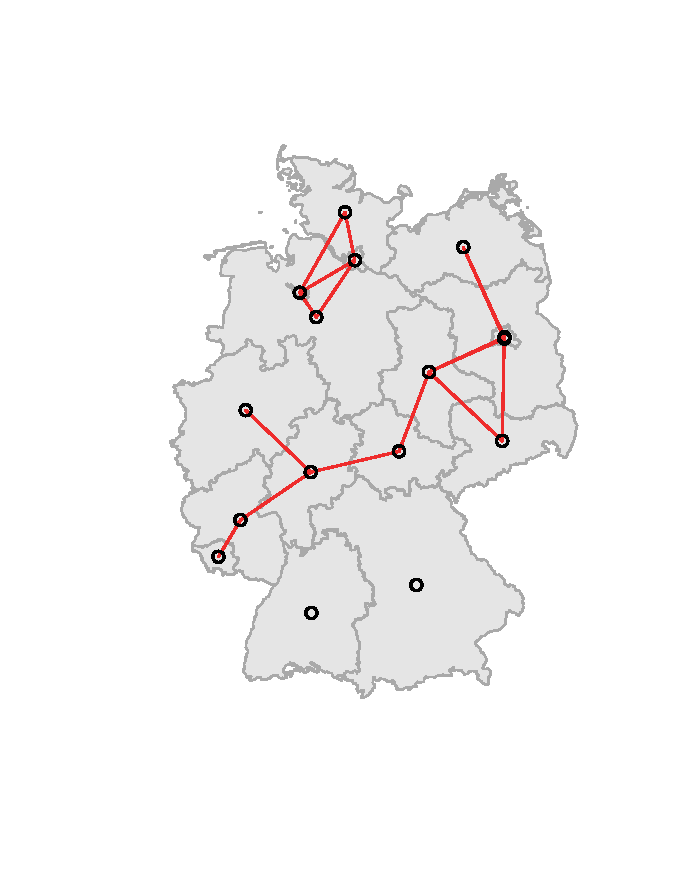
\includegraphics[width=\linewidth,trim={2cm 3cm 1.7cm 2cm},clip]{body/figures/51-BL_nb_d-26k.pdf} % [scale=0.5] oder [width=\linewidth]
       %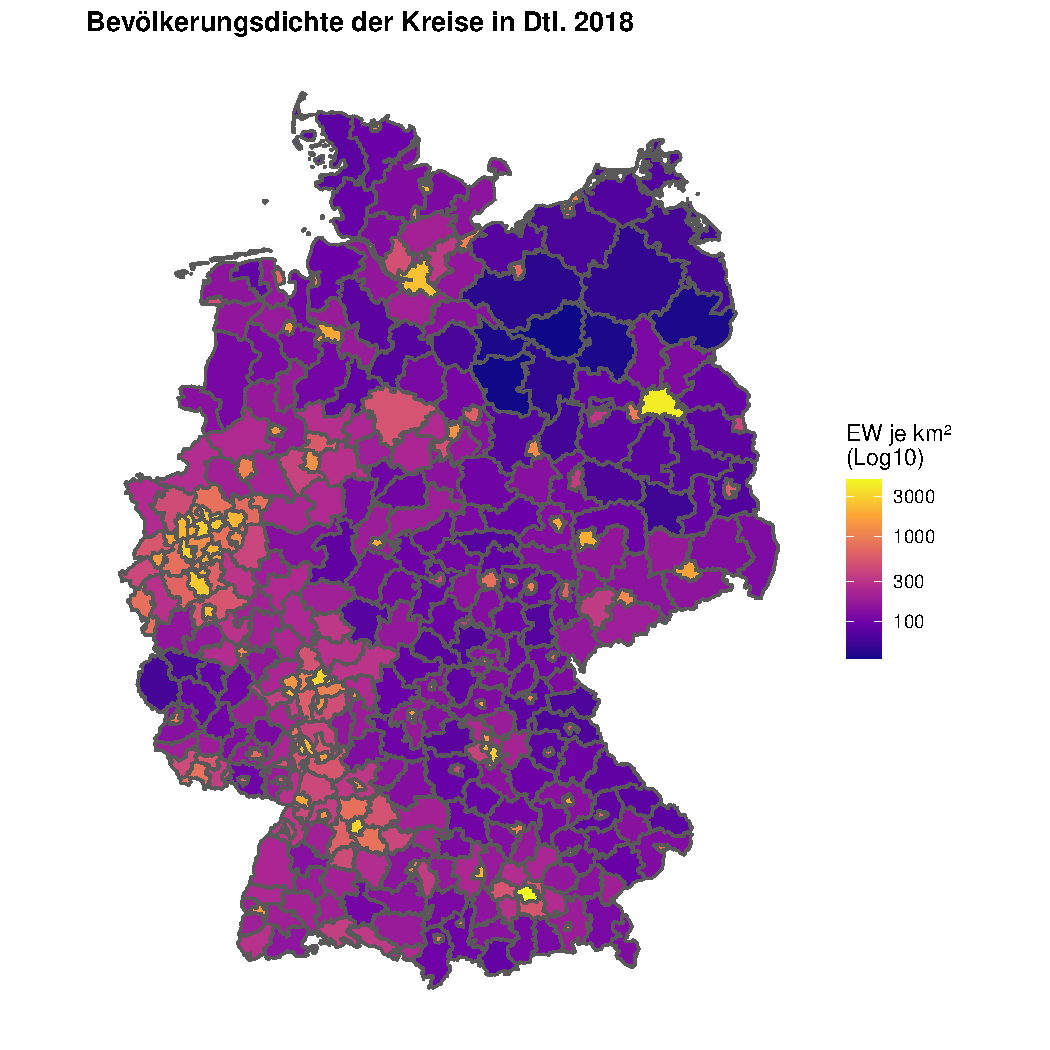
\includegraphics[scale=0.4,trim={1cm 2cm 1cm 2cm},clip]{body/figures/popdens2018.pdf} % [scale=0.5] oder [width=\linewidth]
       %[width=\textwidth] entspricht [width=\linewidth] (=Breite einer Minipage)
       %\caption{erste Nachbarn}
    \end{minipage} % <- sonst wird hier ein Leerzeichen eingefügt
    \hfill
    %\hspace{.1\linewidth}% Abstand zwischen Bilder
    \begin{minipage}[b]{.3\linewidth}
        %\centering
       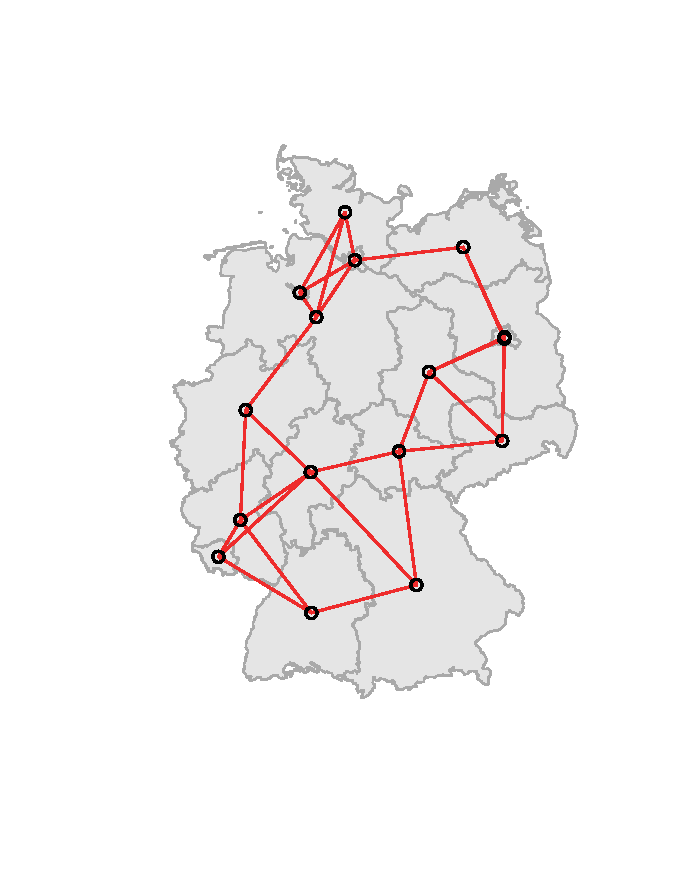
\includegraphics[width=\linewidth,trim={2cm 3cm 1.7cm 2cm},clip]{body/figures/52-BL_nb_k-3.pdf}
       %\caption{zweite Nachbarn}
    \end{minipage}
    \hfill
    %\hspace{.1\linewidth}% Abstand zwischen Bilder
    \begin{minipage}[b]{.3\linewidth}
        %\centering
       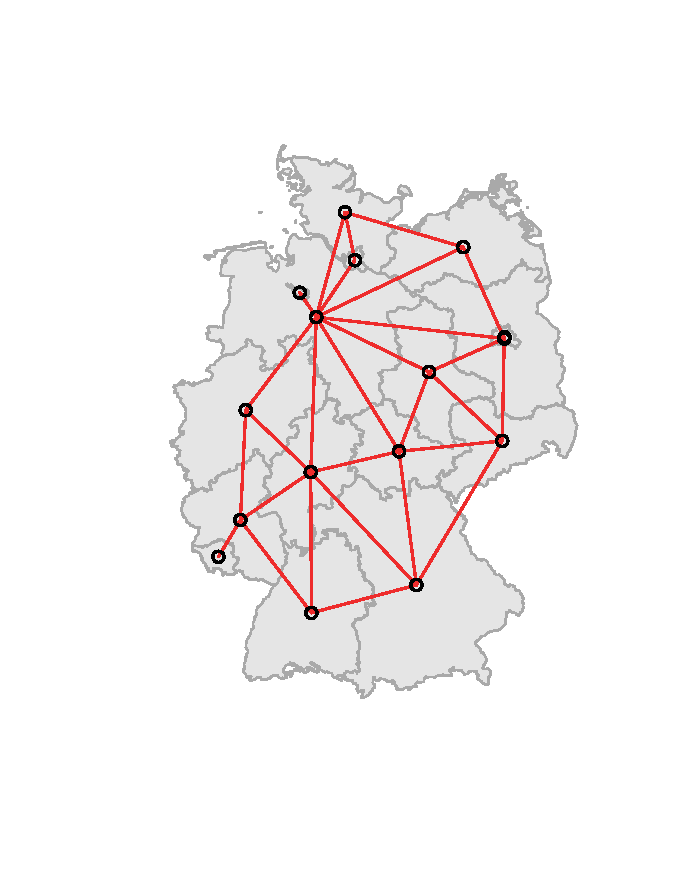
\includegraphics[width=\linewidth,trim={2cm 3cm 1.7cm 2cm},clip]{body/figures/53-BL_nb_qc.pdf}
       %\caption{zweite Nachbarn}
    \end{minipage}
    \caption[Nachbarschaftsgraph]{Nachbarschaftsgraph auf irregulärem Gitter am Bsp der Bundesländer. 
    V.l.n.r.: Distanz $<$ 260km, Drei nächste Nachbarn, Gemeinsame Grenze}
    \label{fig_neighbourgraphs}
 \end{figure}

Nach der Konstruktion der Nachbarschaftsrelation können einzelne Nachbarn geeignet gewichtet werden. 
Bivand et al. (2013, Kapitel 9.2.2) raten jedoch bei geringer Kenntnis über den zugrundeliegenden 
räumlichen Prozess davon ab, von einer binären Repräsentation abzuweichen.

% Fahrmeier nachreichen

Dieses System/Konzept der Nachbarschaftsrelation ist erweiterbar auf zweite und weitere Stufen der Nachbarschaft. 
Über Distanzintervalle $\left(0,d1\right],\left[d1,d2\right],\ldots$ usw. definieren sich erste Nachbarn innerhalb 
der Distanz $d1$ von $i$. Zweite Nachbarn sind innerhalb des Entfernungsbandes von $d1$ bis $d2$ lokalisiert.


\begin{figure} %[htb] %h=here, t=top, b=bottom, p=page of float
    \centering %Bilder mittig statt am linken Rand ausgerichtet
    \begin{minipage}[b]{.22\linewidth} % [b] => Ausrichtung an \caption --> c (=Center) t (=Top) und b (=Bottom)
        % \linewidth entspricht hier \textwidth (=Breite Textbereich)
        %\centering
        %                                 trim = links unten rechts oben
        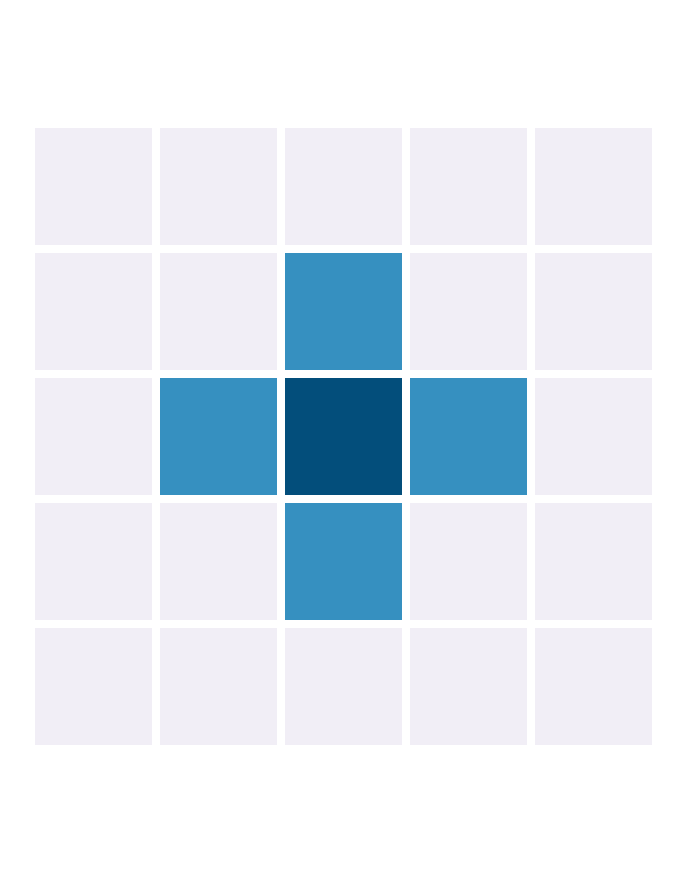
\includegraphics[width=\linewidth,trim={0.7cm 2.2cm 0.7cm 2.2cm},clip]{body/figures/61-nb_e.pdf} % [scale=0.5] oder [width=\linewidth]
       %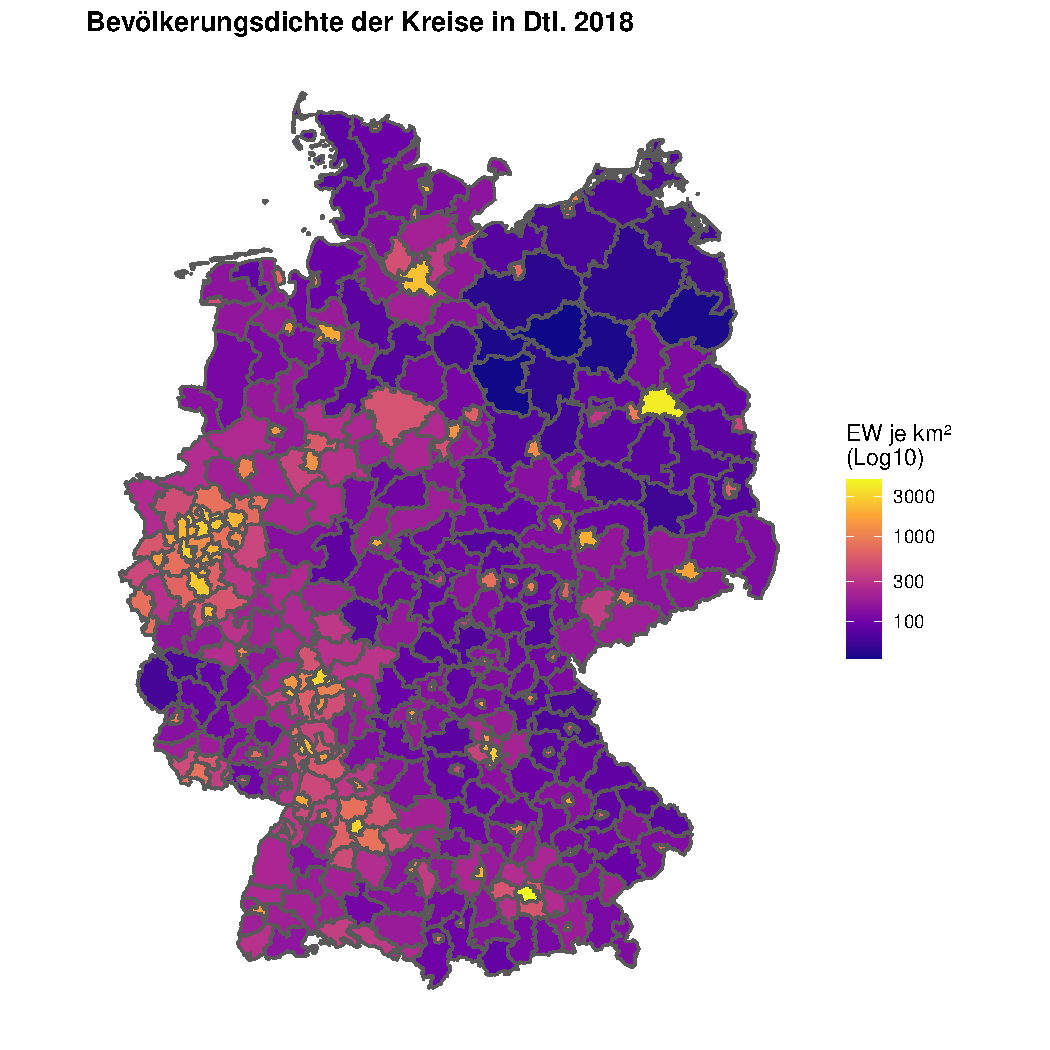
\includegraphics[scale=0.4,trim={1cm 2cm 1cm 2cm},clip]{body/figures/popdens2018.pdf} % [scale=0.5] oder [width=\linewidth]
       %[width=\textwidth] entspricht [width=\linewidth] (=Breite einer Minipage)
       %\caption{erste Nachbarn}
    \end{minipage} % <- sonst wird hier ein Leerzeichen eingefügt
    \hfill
    %\hspace{.1\linewidth}% Abstand zwischen Bilder
    \begin{minipage}[b]{.22\linewidth}
        %\centering
       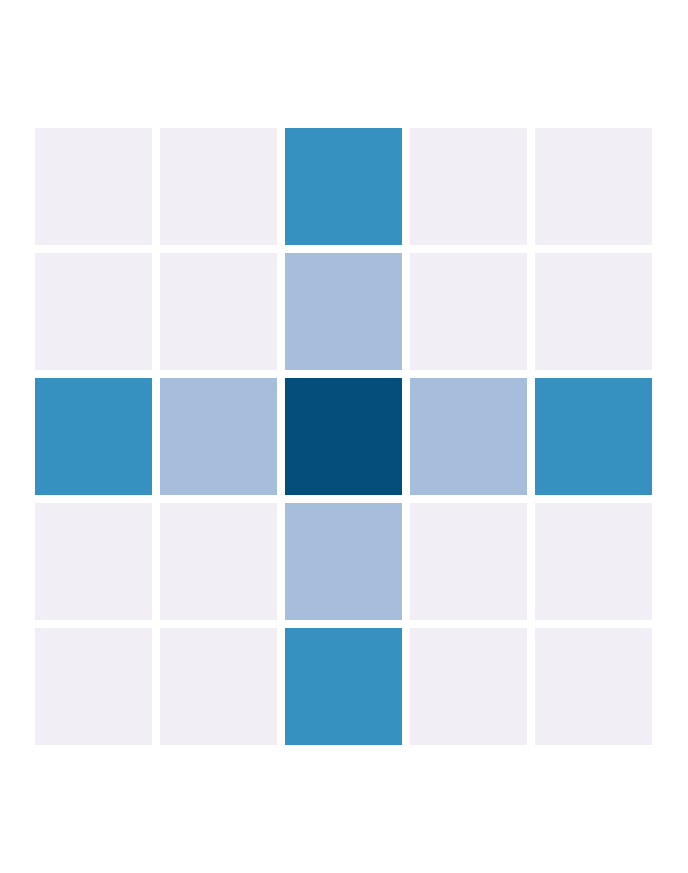
\includegraphics[width=\linewidth,trim={0.7cm 2.2cm 0.7cm 2.2cm},clip]{body/figures/62-nb_z.pdf}
       %\caption{zweite Nachbarn}
    \end{minipage}
    \hfill
    %\hspace{.1\linewidth}% Abstand zwischen Bilder
    \begin{minipage}[b]{.22\linewidth}
        %\centering
       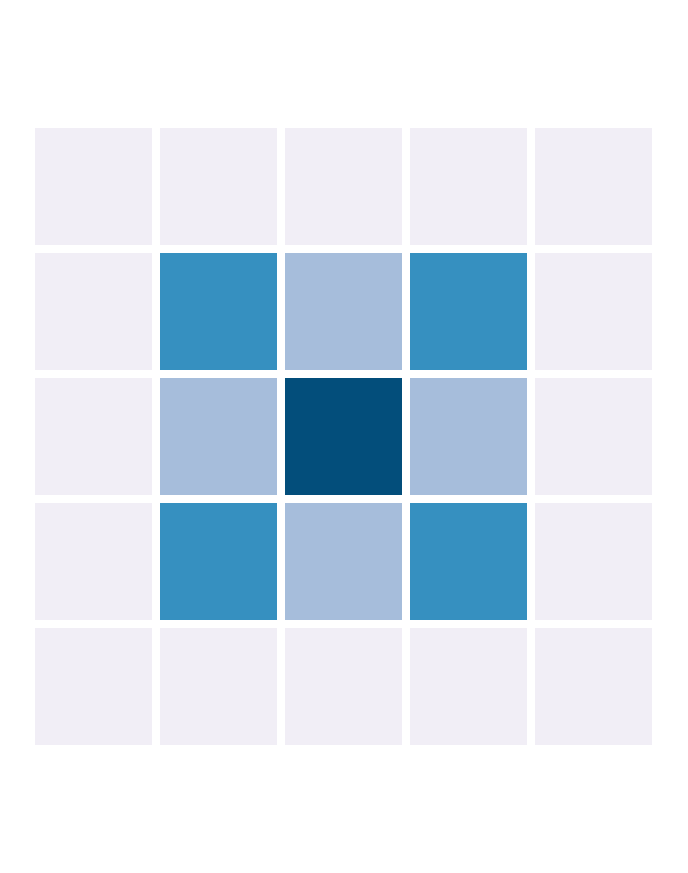
\includegraphics[width=\linewidth,trim={0.7cm 2.2cm 0.7cm 2.2cm},clip]{body/figures/63-nb_d.pdf}
       %\caption{zweite Nachbarn}
    \end{minipage}
    \hfill
    %\hspace{.1\linewidth}% Abstand zwischen Bilder
    \begin{minipage}[b]{.22\linewidth}
        %\centering
       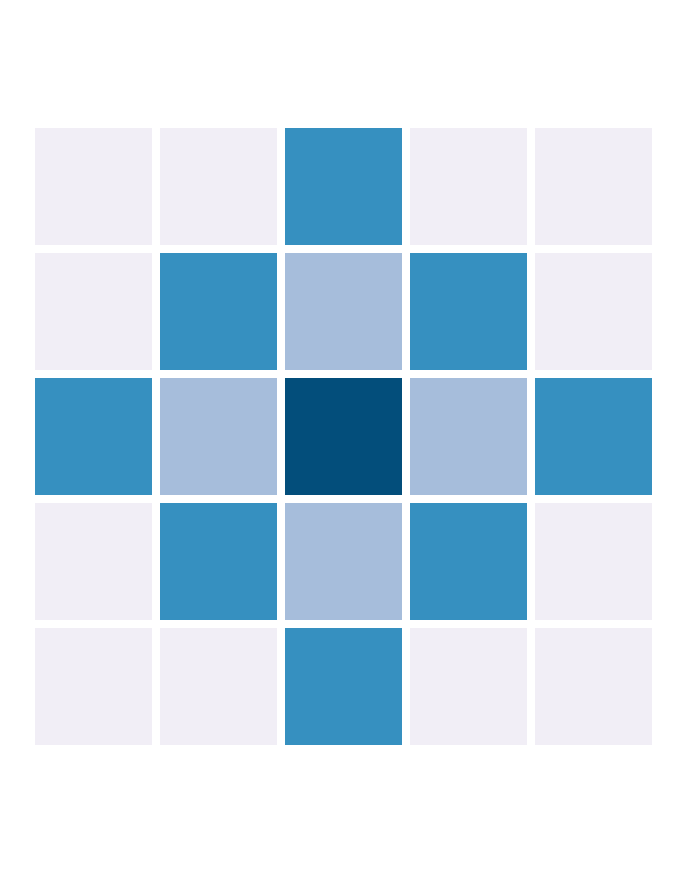
\includegraphics[width=\linewidth,trim={0.7cm 2.2cm 0.7cm 2.2cm},clip]{body/figures/64-nb_zd.pdf}
       %\caption{zweite Nachbarn}
    \end{minipage}
    \caption[Nachbarschaftssysteme]{Nachbarschaftssystem auf regulärem Gitter. V.l.n.r.: Erste, zweite, 
    diagonale, zweite und diagonale Nachbarn}
    \label{fig_neighbours}
 \end{figure}


In Abbildung \ref{fig_neighbours} sind verschiedene Nachbarschaftssysteme für ein reguläres 
(Raster?)Gitter (exemplarisch) bezüglich 
gemeinsamer Grenzen (entspricht Manhattan-Distanz?) dargestellt. In Abbildung \ref{fig_neighbours_bl} die Anwendung auf ein 
irreguläres Gitter der Gebiete deutscher Bundesländer mit $s_i=\text{Thüringen}$.

\begin{figure} %[htb] %h=here, t=top, b=bottom, p=page of float
    \centering %Bilder mittig statt am linken Rand ausgerichtet
    \begin{minipage}[b]{.3\linewidth} % [b] => Ausrichtung an \caption --> c (=Center) t (=Top) und b (=Bottom)
        % \linewidth entspricht hier \textwidth (=Breite Textbereich)
        %\centering
        %                                 trim = links unten rechts oben
        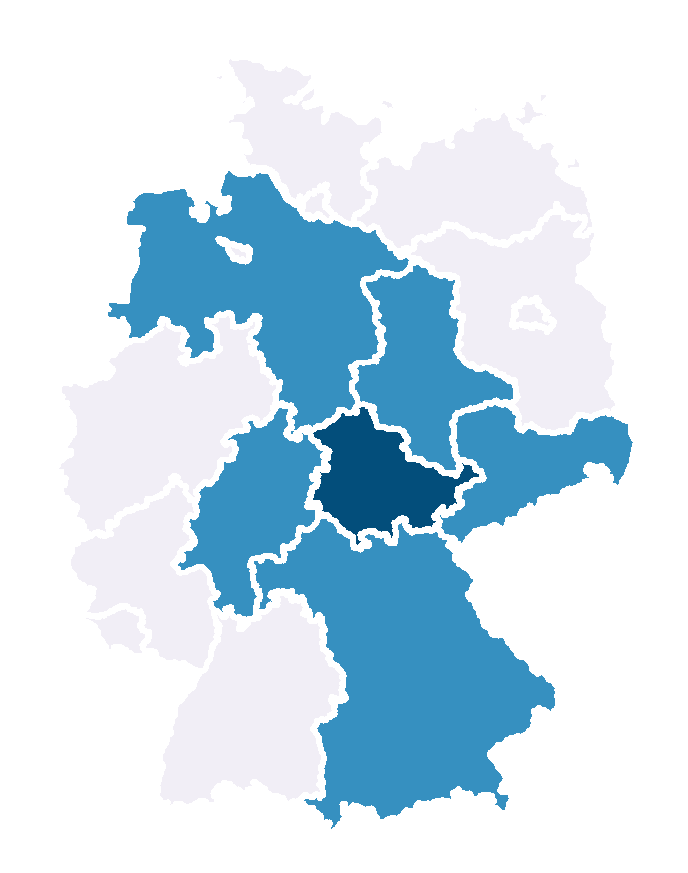
\includegraphics[width=\linewidth,trim={1cm 1cm 1cm 1cm},clip]{body/figures/71-BL_nb_e.pdf} % [scale=0.5] oder [width=\linewidth]
       %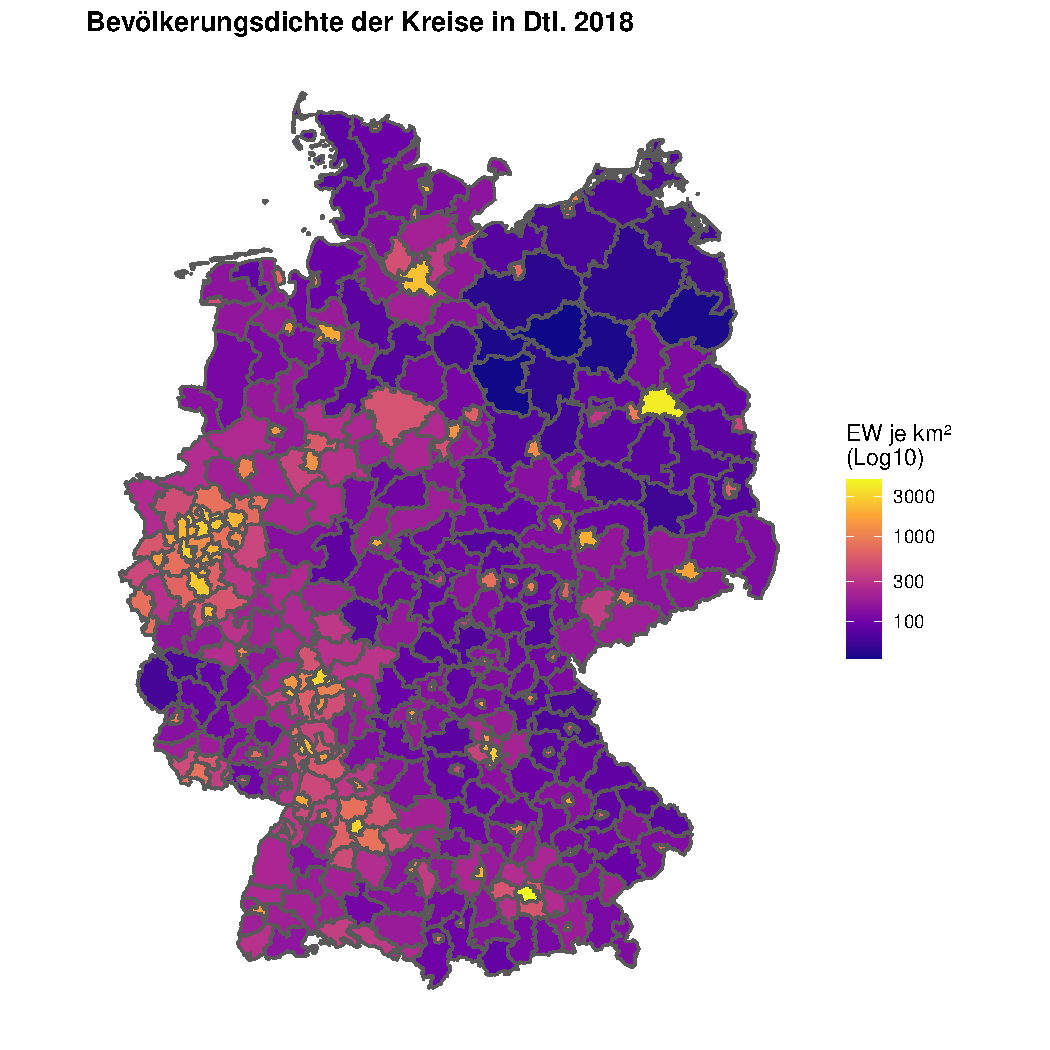
\includegraphics[scale=0.4,trim={1cm 2cm 1cm 2cm},clip]{body/figures/popdens2018.pdf} % [scale=0.5] oder [width=\linewidth]
       %[width=\textwidth] entspricht [width=\linewidth] (=Breite einer Minipage)
       %\caption{erste Nachbarn}
    \end{minipage} % <- sonst wird hier ein Leerzeichen eingefügt
    \hfill
    %\hspace{.1\linewidth}% Abstand zwischen Bilder
    \begin{minipage}[b]{.3\linewidth}
        %\centering
       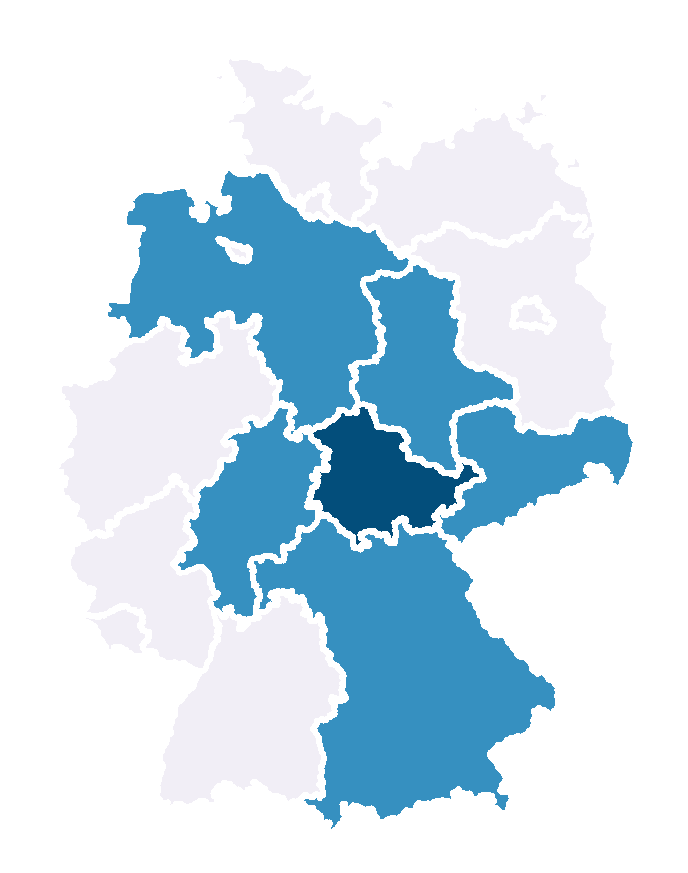
\includegraphics[width=\linewidth,trim={1cm 1cm 1cm 1cm},clip]{body/figures/71-BL_nb_e.pdf}
       %\caption{zweite Nachbarn}
    \end{minipage}
    \hfill
    %\hspace{.1\linewidth}% Abstand zwischen Bilder
    \begin{minipage}[b]{.3\linewidth}
        %\centering
       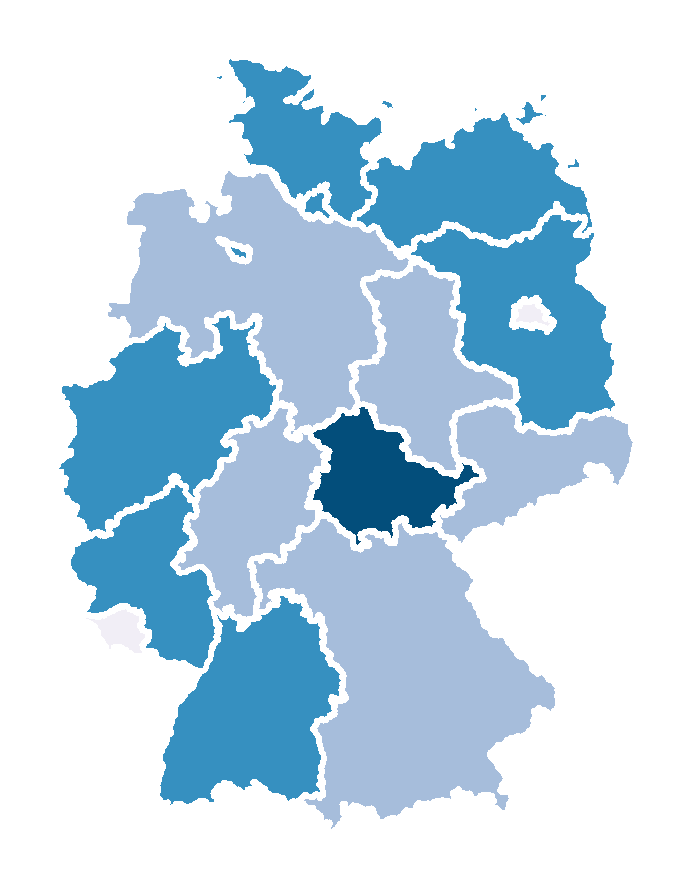
\includegraphics[width=\linewidth,trim={1cm 1cm 1cm 1cm},clip]{body/figures/73-BL_nb_zd.pdf}
       %\caption{zweite Nachbarn}
    \end{minipage}
    \caption[Nachbarschaftssysteme]{Nachbarschaftssystem auf irregulärem Gitter am Bsp der Bundesländer. 
    V.l.n.r.: Erste, zweite, diagonale}
    \label{fig_neighbours_bl}
 \end{figure}

Nachbarschaftsmatrix W wird entsprechend Kapitel 4.XX konstruiert und speichert im folgenden alle Nachbarschaftsinformationen. 
Die Einträge $w_{ij}$ entsprechen den Gewichten. Dabei werden Diagonaleinträge $w_{ii}$ auf Null gesetzt. 
In einer Standardisierung werden die Einträge der Zeile $i$ durch Zeilensumme $\sum_{j=1}^{n} w_{ij}$ geteilt.

Analog zur Erweiterung des Nachbarschaftssystems/graphen kann die Nachbarschaftsmatrix W1, W2 usw. 
mit Nachbarschaftsrelationen ersten bzw zweiten Grades gebildet werden.
